\chapter{Extended Control Results }
\label{Control_Results}
This appendix contains the corresponding plots of the ISTTOK discharges from table \ref{TableControl}.

\begin{figure}[h]
	\centering
	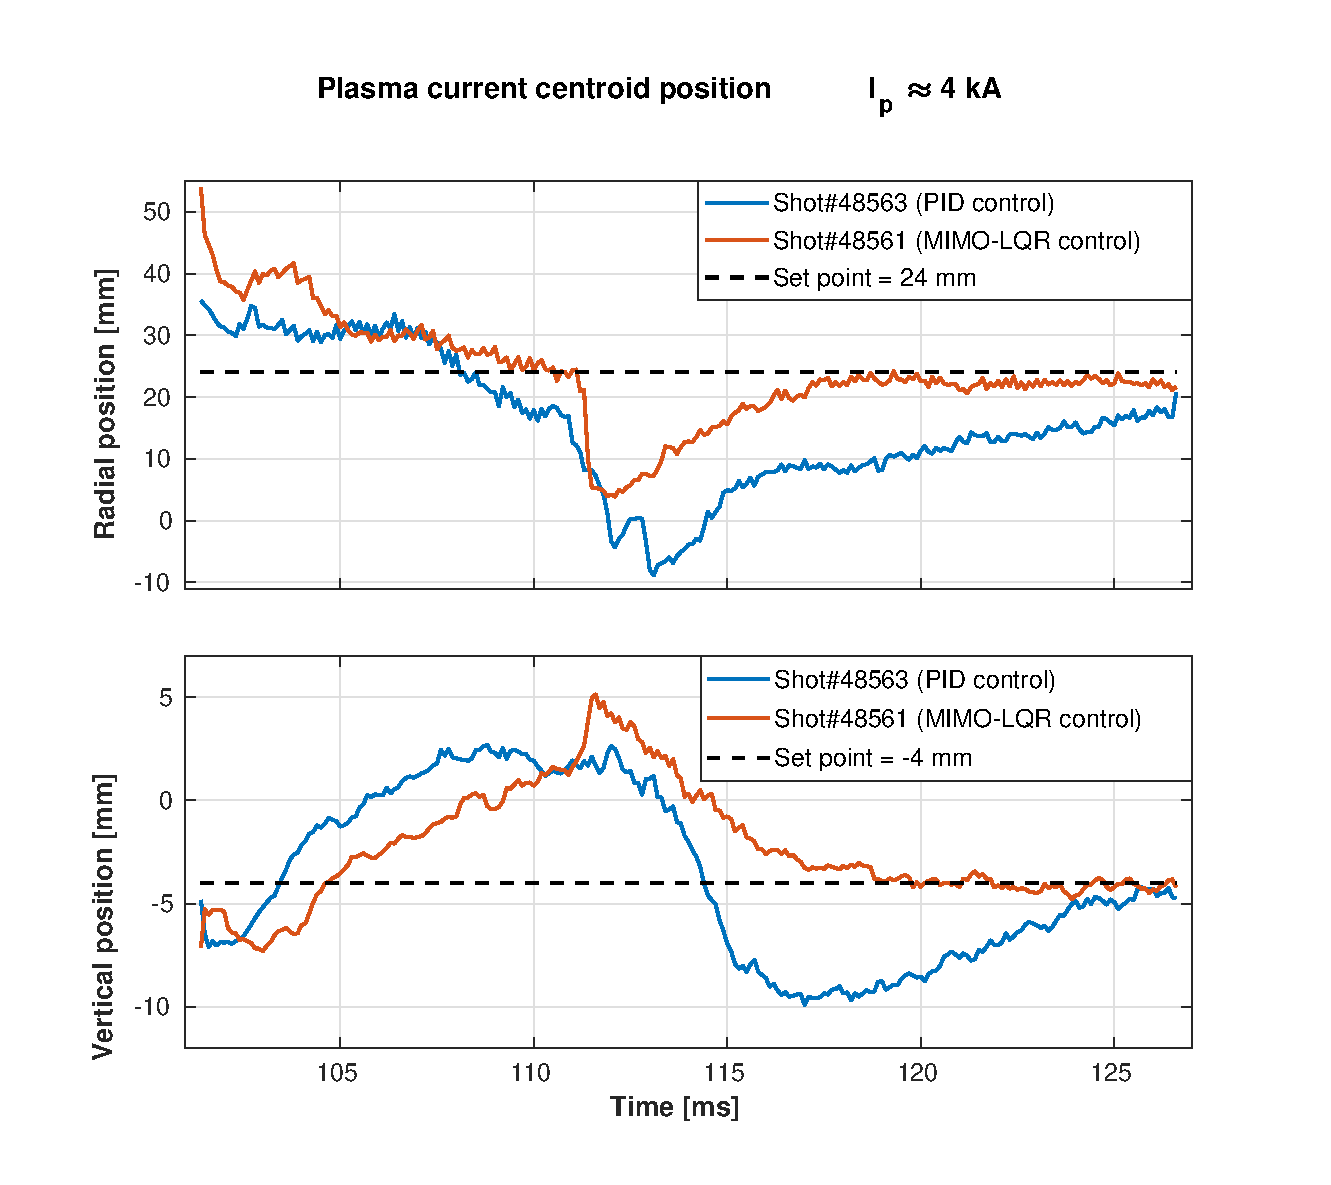
\includegraphics[width=0.7\textwidth]{Chp5/PIDvsMIMO_563_561_2.eps}
	\caption{Horizontal and vertical plasma centroid position during  $I_p\approx 4kA$  flat-tops, orange time trace corresponds to a PID feedback control and blue time trace to a LQR MIMO feedback control, the dashed black line shows the programmed set point. Shot$\#$ 48563 and Shot$\#$ 48561.}
\end{figure}

\begin{figure}
	\centering
	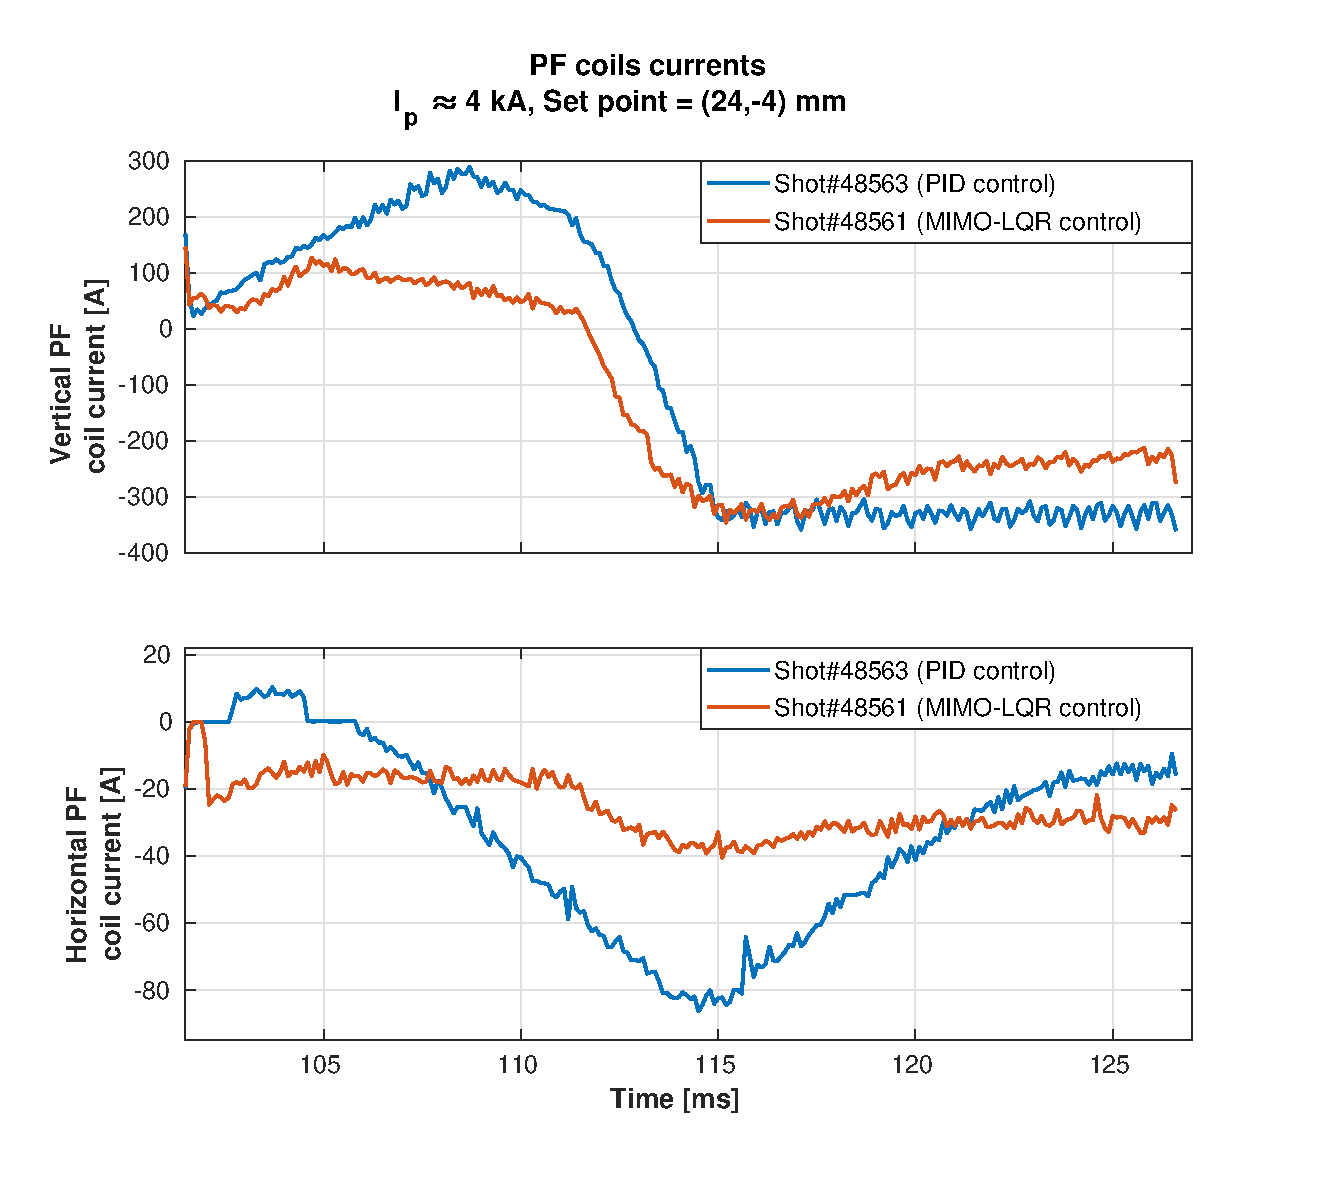
\includegraphics[width=0.7\textwidth]{Chp5/PIDvsMIMO_563_561_curr_2.eps}
	\caption{  Vertical and Horizontal PF coils currents during  $I_p\approx 4kA$  flat-tops. Orange time trace corresponds to a PID feedback control and blue time trace to a LQR MIMO feedback control. Shot $\#$ 48563 and Shot $\#$ 48561.}
\end{figure}

\begin{figure}
	\centering
	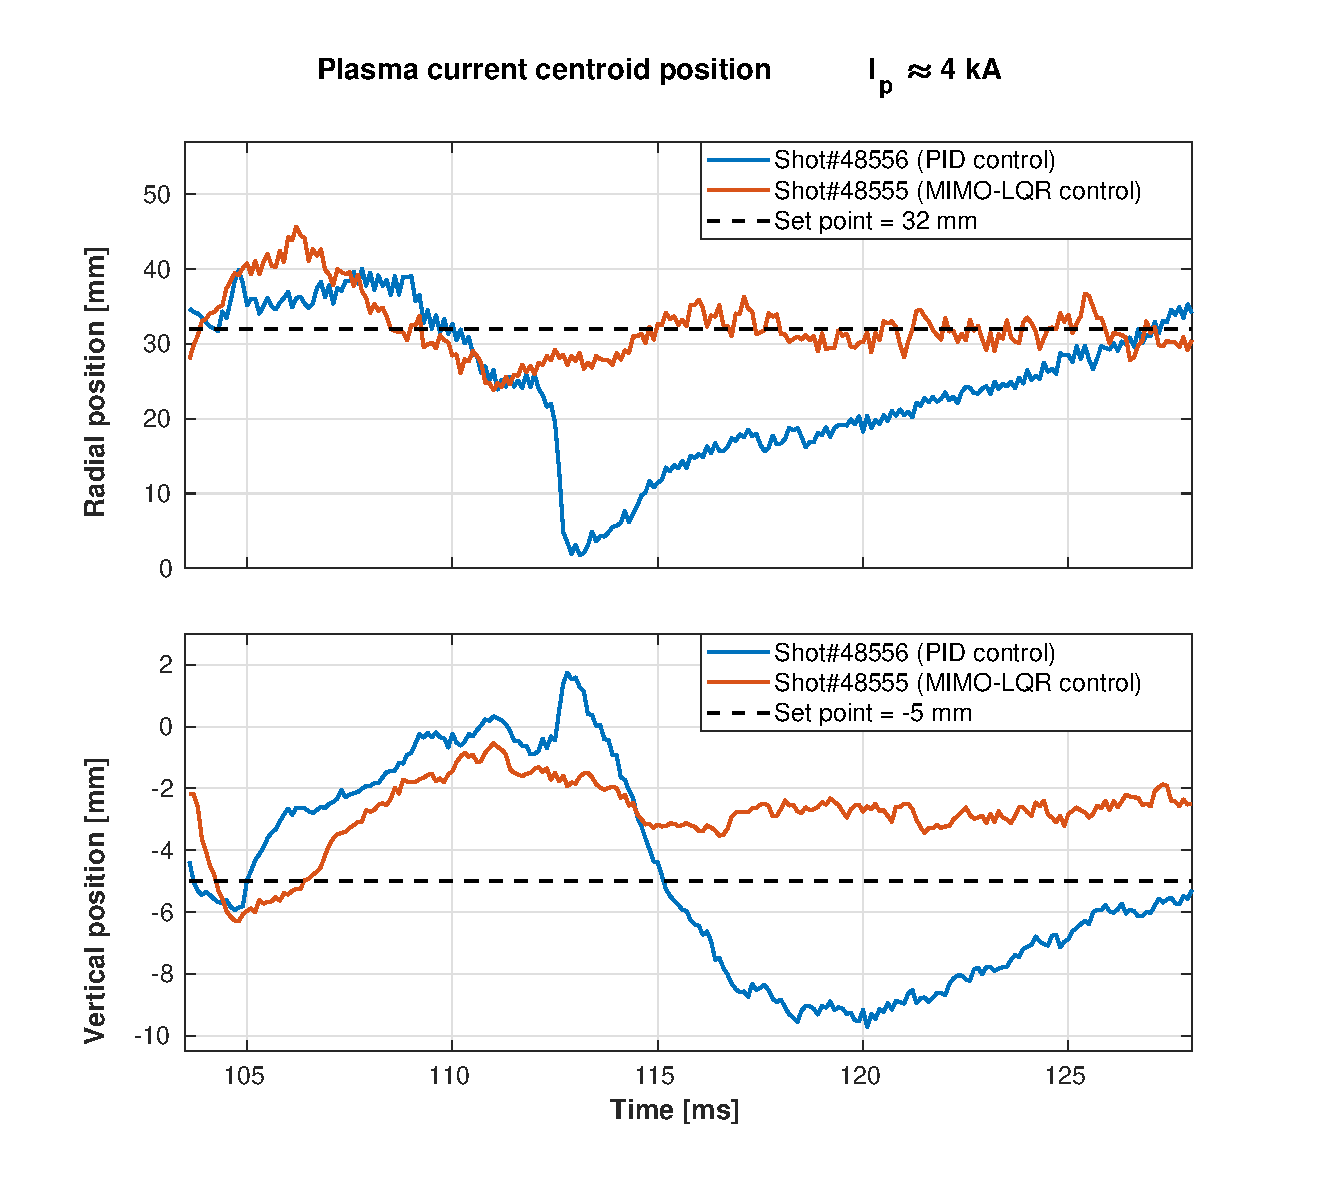
\includegraphics[width=0.7\textwidth]{Chp5/PIDvsMIMO_556_555_2.eps}
	\caption{Horizontal and vertical plasma centroid position during  $I_p\approx 4kA$  flat-tops, orange time trace corresponds to a PID feedback control and blue time trace to a LQR MIMO feedback control, the dashed black line shows the programmed set point. Shot $\#$ 48556 and Shot $\#$ 48555.}
\end{figure}

\begin{figure}
	\centering
	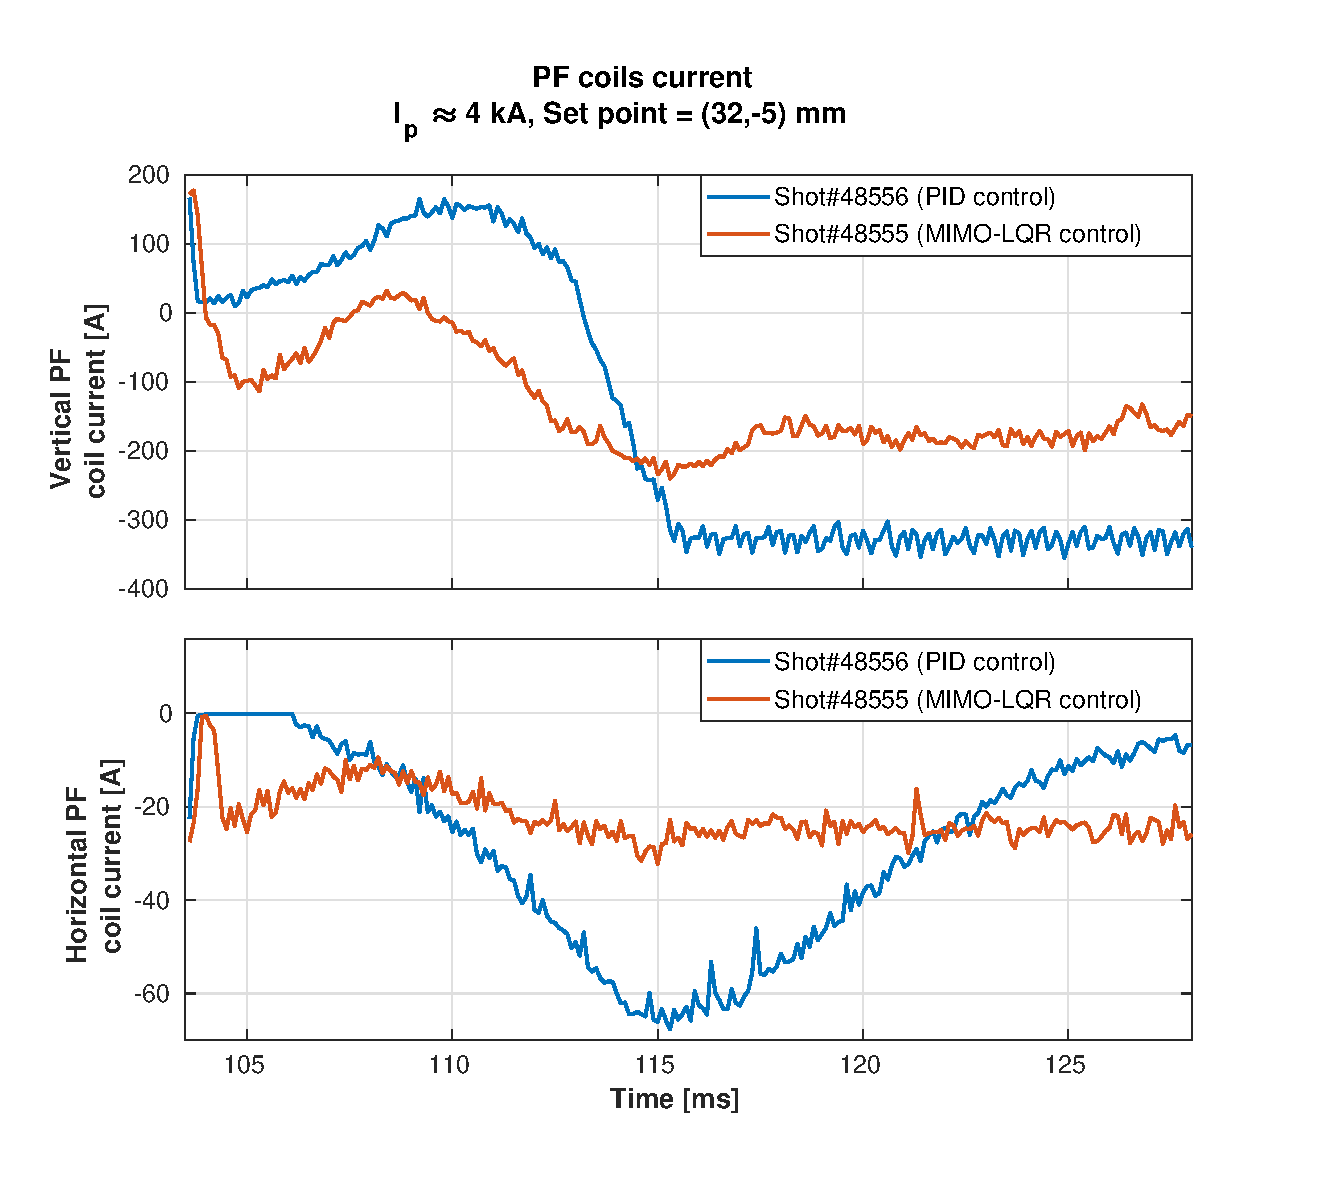
\includegraphics[width=0.7\textwidth]{Chp5/PIDvsMIMO_556_555_curr_2.eps}
	\caption{  Vertical and Horizontal PF coils currents during  $I_p\approx 4kA$  flat-tops. Orange time trace corresponds to a PID feedback control and blue time trace to a LQR MIMO feedback control.  Shot$\#$ 48556 and Shot$\#$ 48555.}
\end{figure}

\begin{figure}
	\centering
	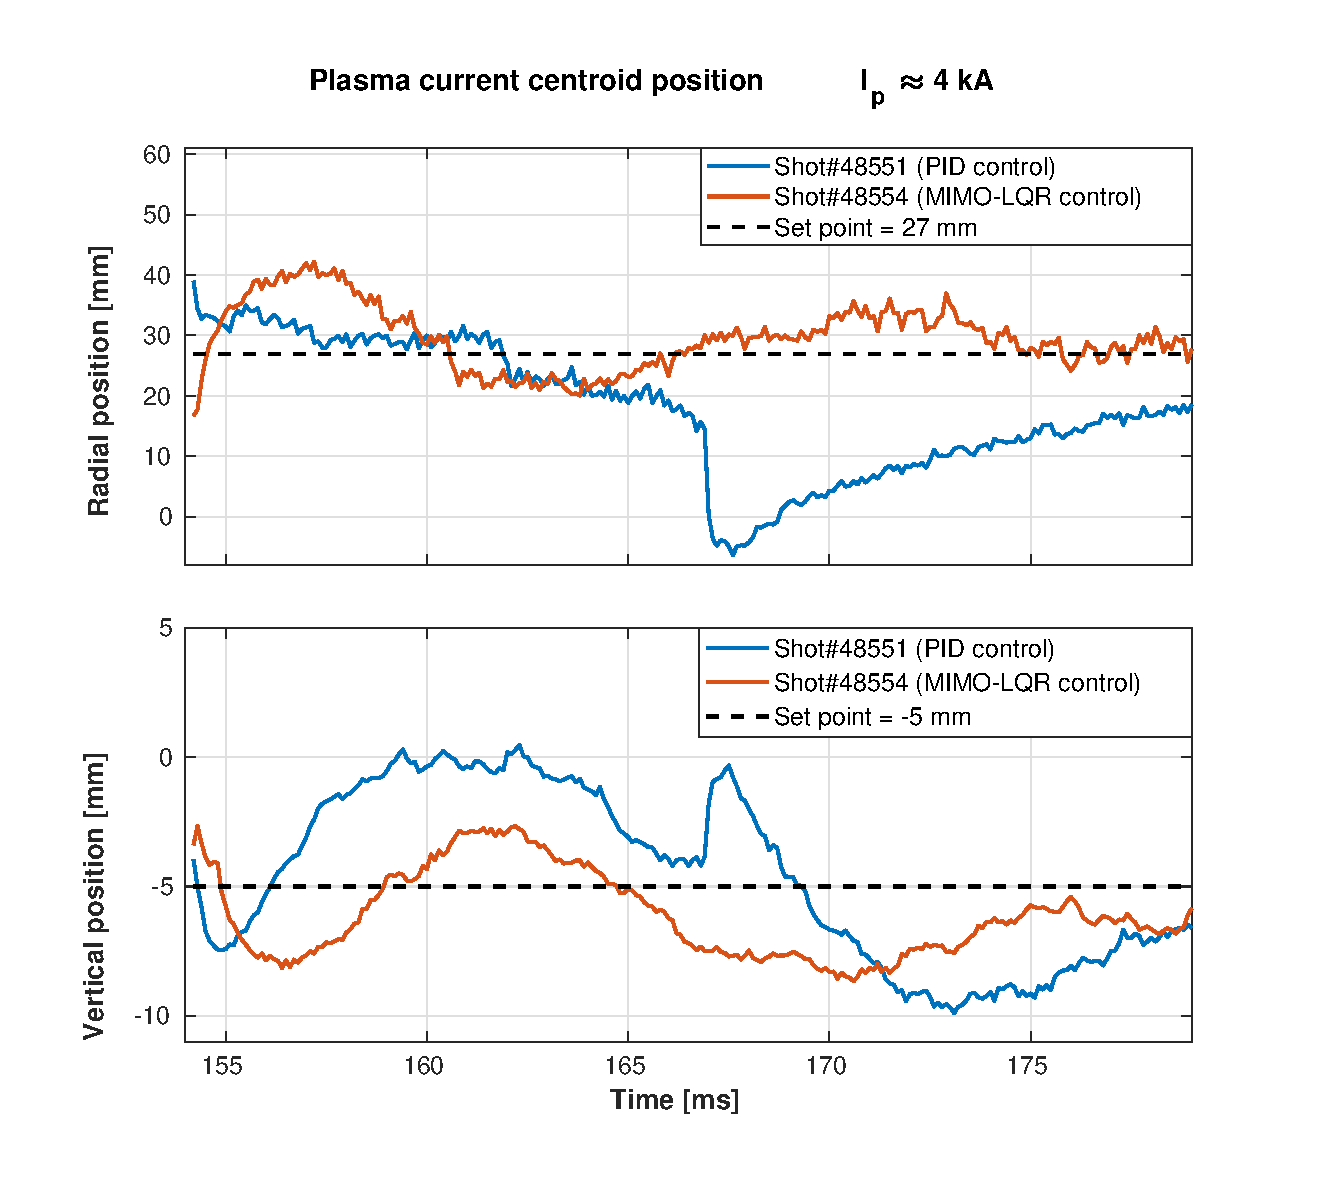
\includegraphics[width=0.7\textwidth]{Chp5/PIDvsMIMO_551_554_2.eps}
	\caption{ Horizontal and vertical plasma centroid position during  $I_p\approx 4kA$  flat-tops, orange time trace corresponds to a PID feedback control and blue time trace to a LQR MIMO feedback control, the dashed black line shows the programmed set point. Shot$\#$ 48551 Shot$\#$ 48554. }
\end{figure}

\begin{figure}
	\centering
	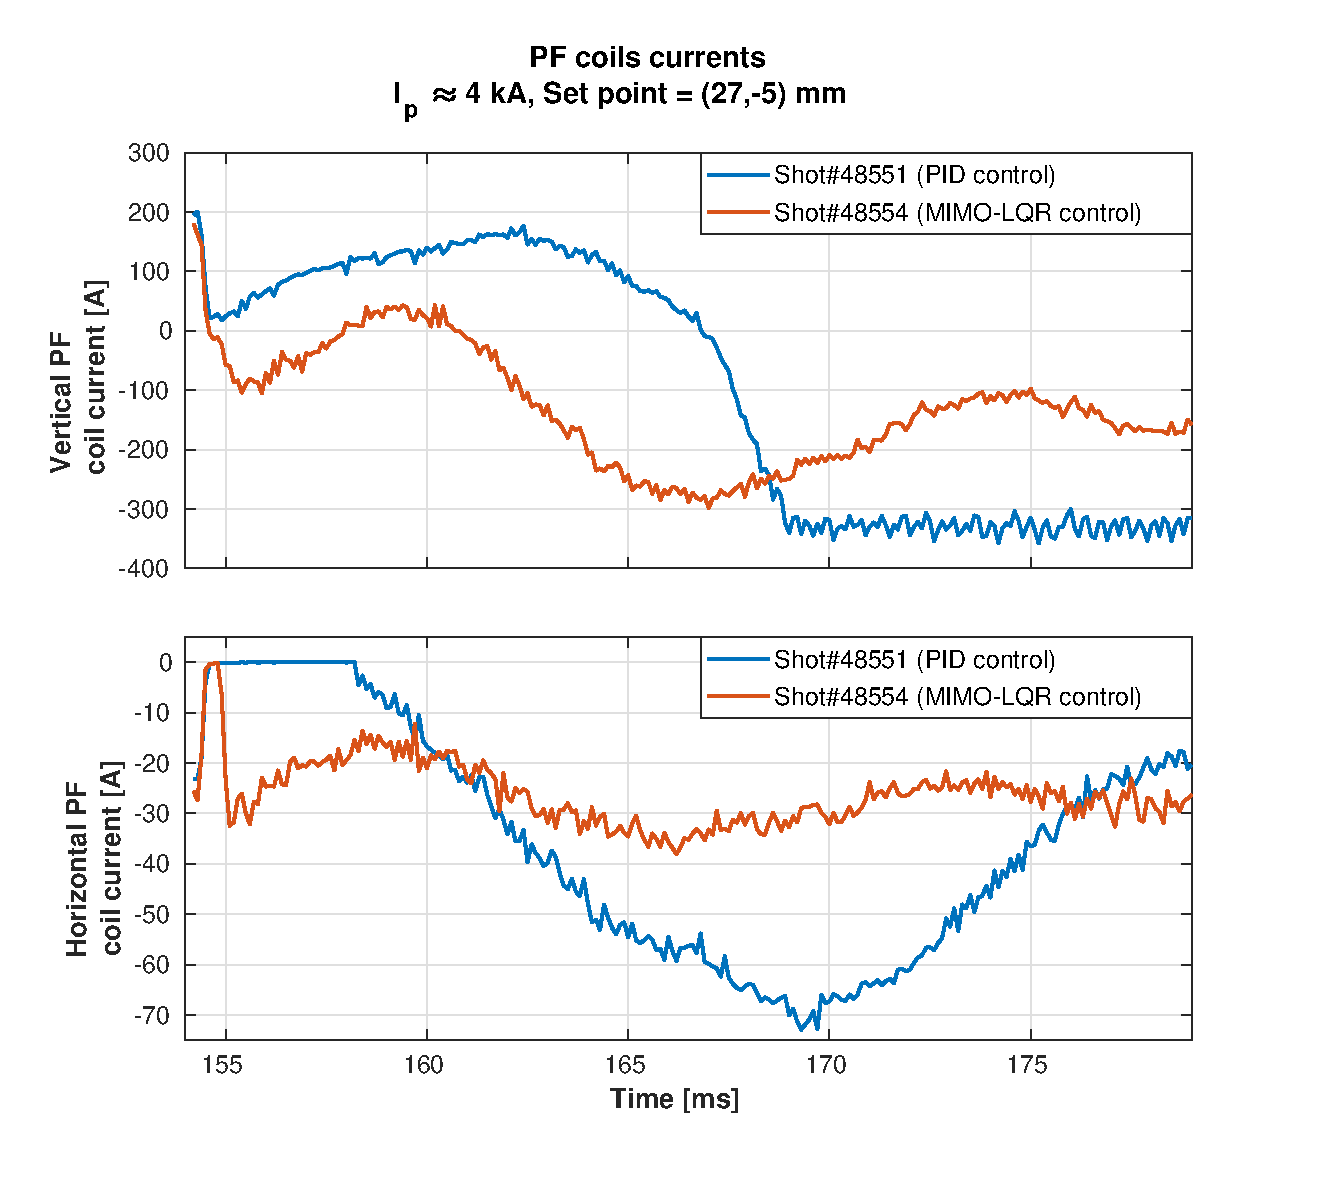
\includegraphics[width=0.7\textwidth]{Chp5/PIDvsMIMO_551_554_curr_2.eps}
	\caption{   Vertical and Horizontal PF coils currents during  $I_p\approx 4kA$  flat-tops. Orange time trace corresponds to a PID feedback control and blue time trace to a LQR MIMO feedback control.  Shot$\#$ 48551 and Shot$\#$ 48554.}
\end{figure}
\begin{figure}
	\centering
	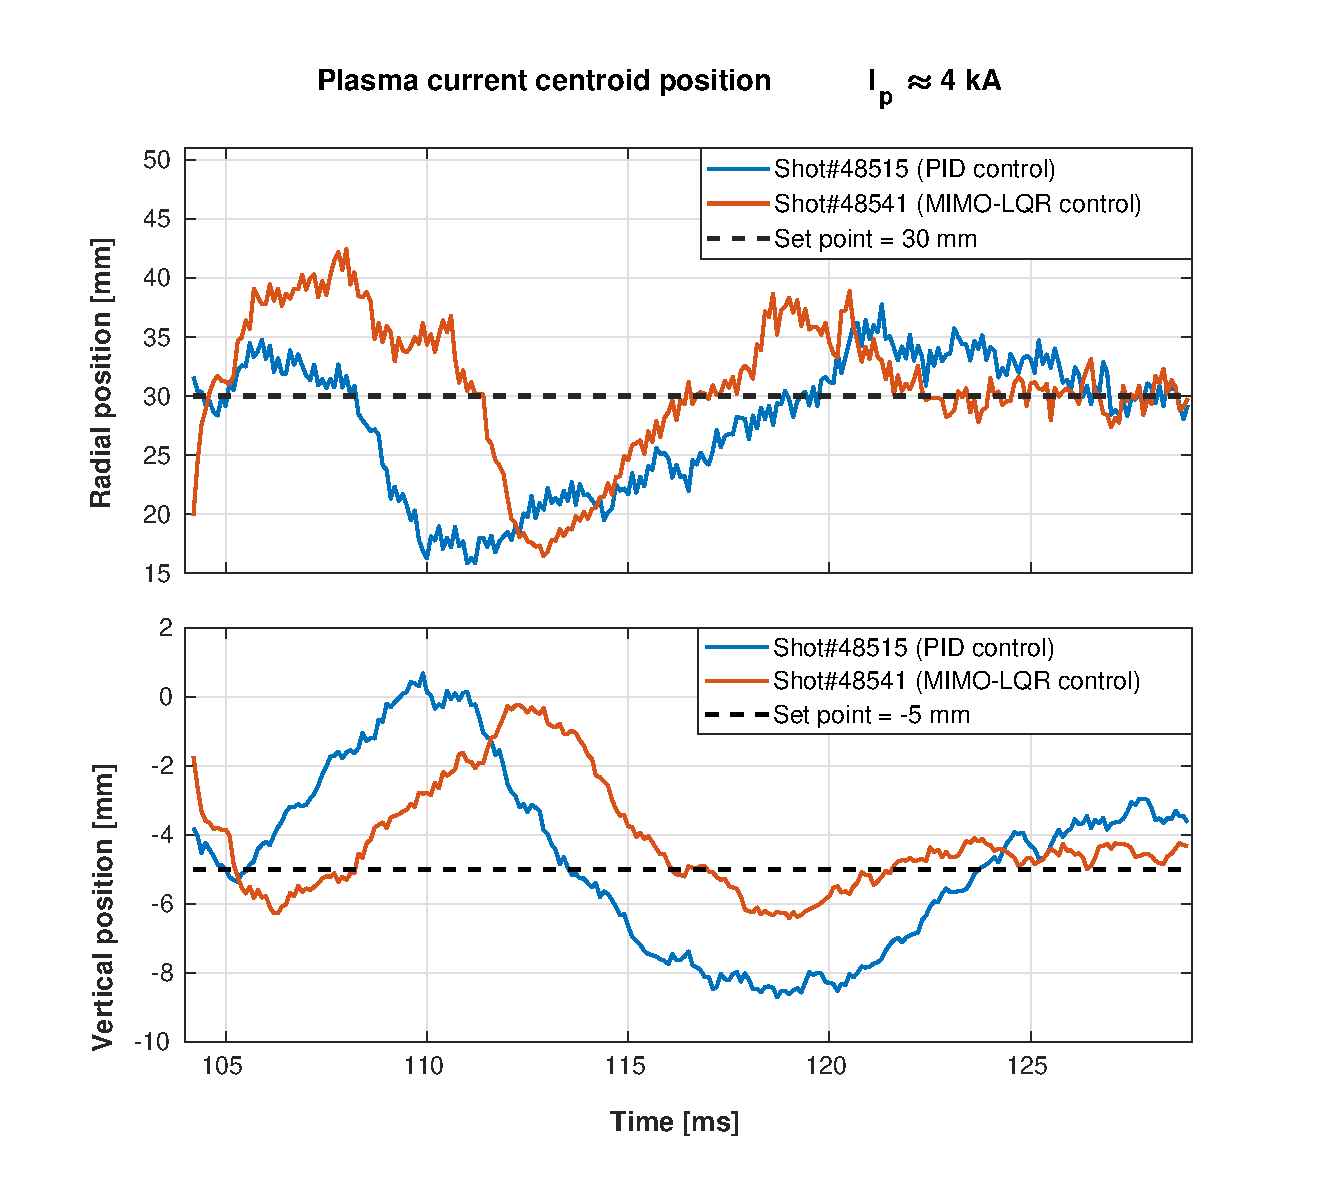
\includegraphics[width=0.7\textwidth]{Chp5/PIDvsMIMO_515_541_2.eps}
	\caption{Horizontal and vertical plasma centroid position during  $I_p\approx 4kA$  flat-tops, orange time trace corresponds to a PID feedback control and blue time trace to a LQR MIMO feedback control, the dashed black line shows the programmed set point.  Shot$\#$ 48515 and Shot$\#$ 48541.}
\end{figure}

\begin{figure}
	\centering
	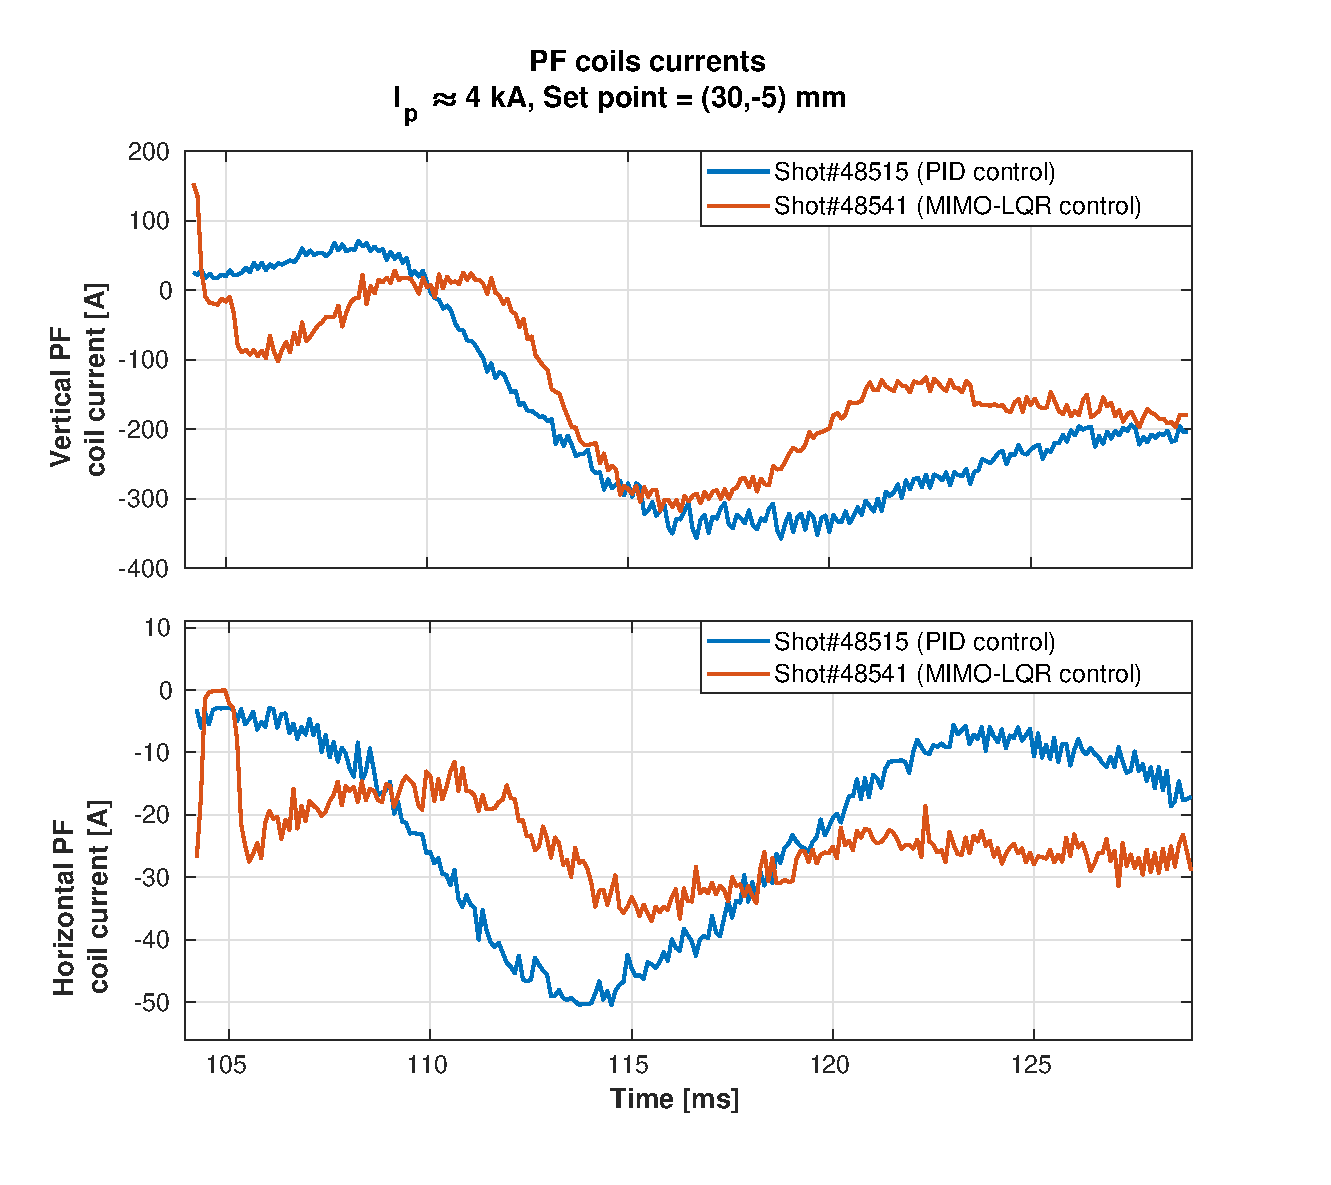
\includegraphics[width=0.7\textwidth]{Chp5/PIDvsMIMO_515_541_curr_2.eps}
	\caption{   Vertical and Horizontal PF coils currents during  $I_p\approx 4kA$  flat-tops. Orange time trace corresponds to a PID feedback control and blue time trace to a LQR MIMO feedback control. Shot$\#$ 48515 and Shot$\#$ 48541.}
\end{figure}

\begin{figure}
	\centering
	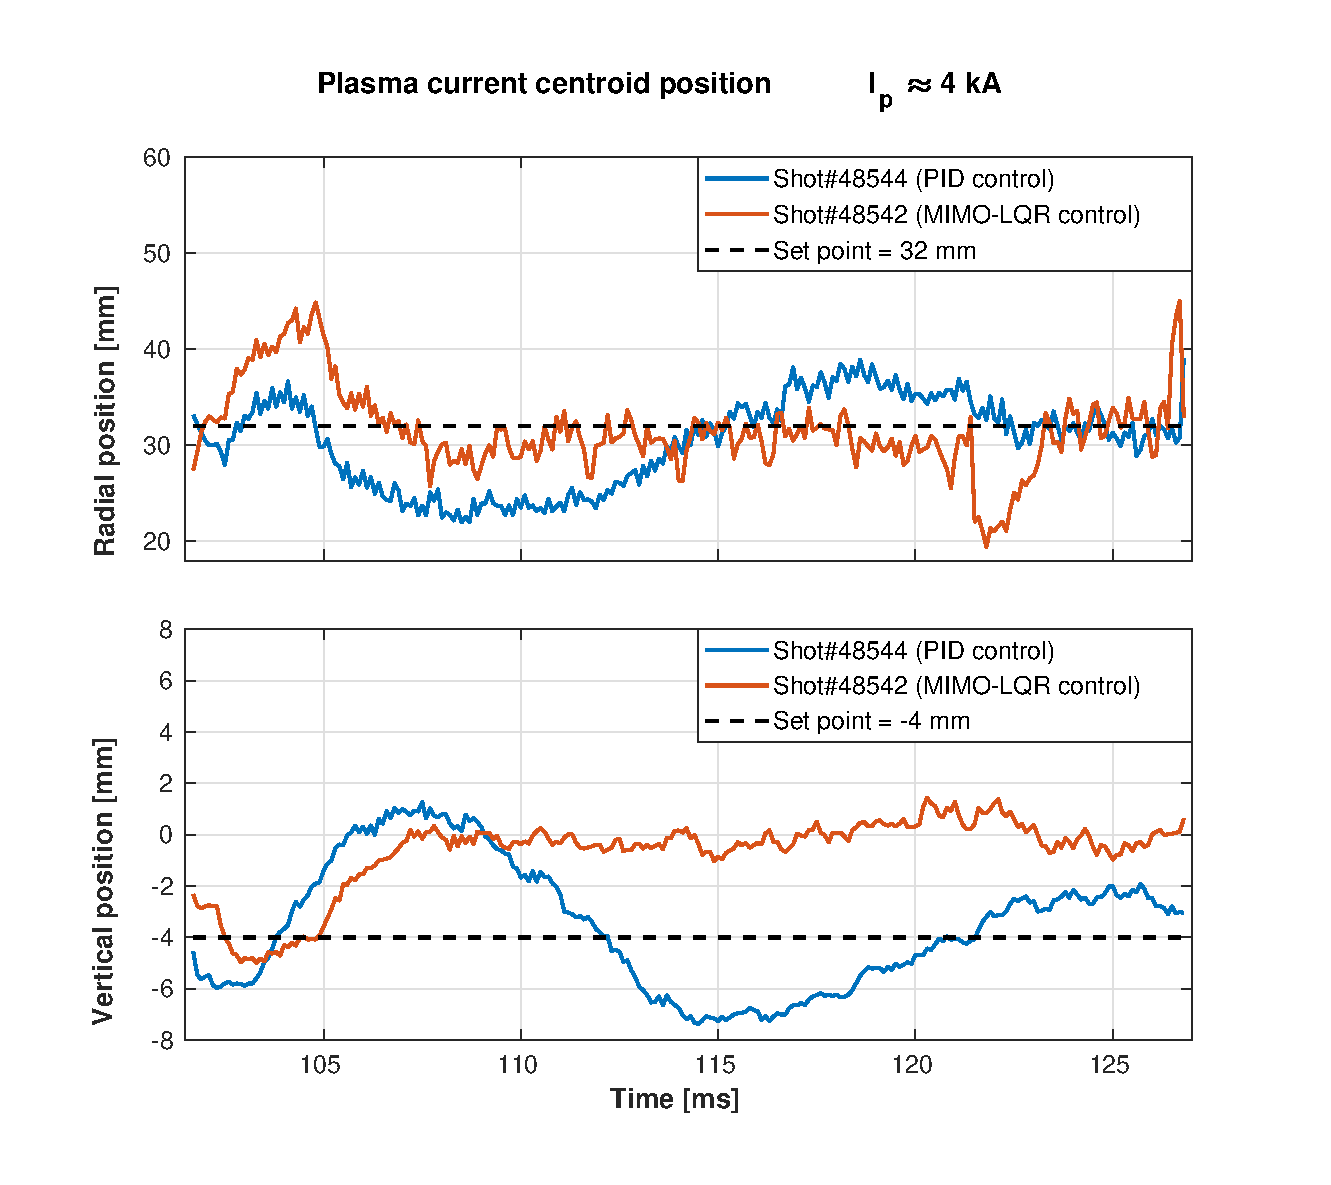
\includegraphics[width=0.7\textwidth]{Chp5/PIDvsMIMO_544_542_2.eps}
	\caption{Horizontal and vertical plasma centroid position during  $I_p\approx 4kA$  flat-tops, orange time trace corresponds to a PID feedback control and blue time trace to a LQR MIMO feedback control, the dashed black line shows the programmed set point.   Shot$\#$ 48544 and Shot$\#$ 48542.}
\end{figure}

\begin{figure}
	\centering
	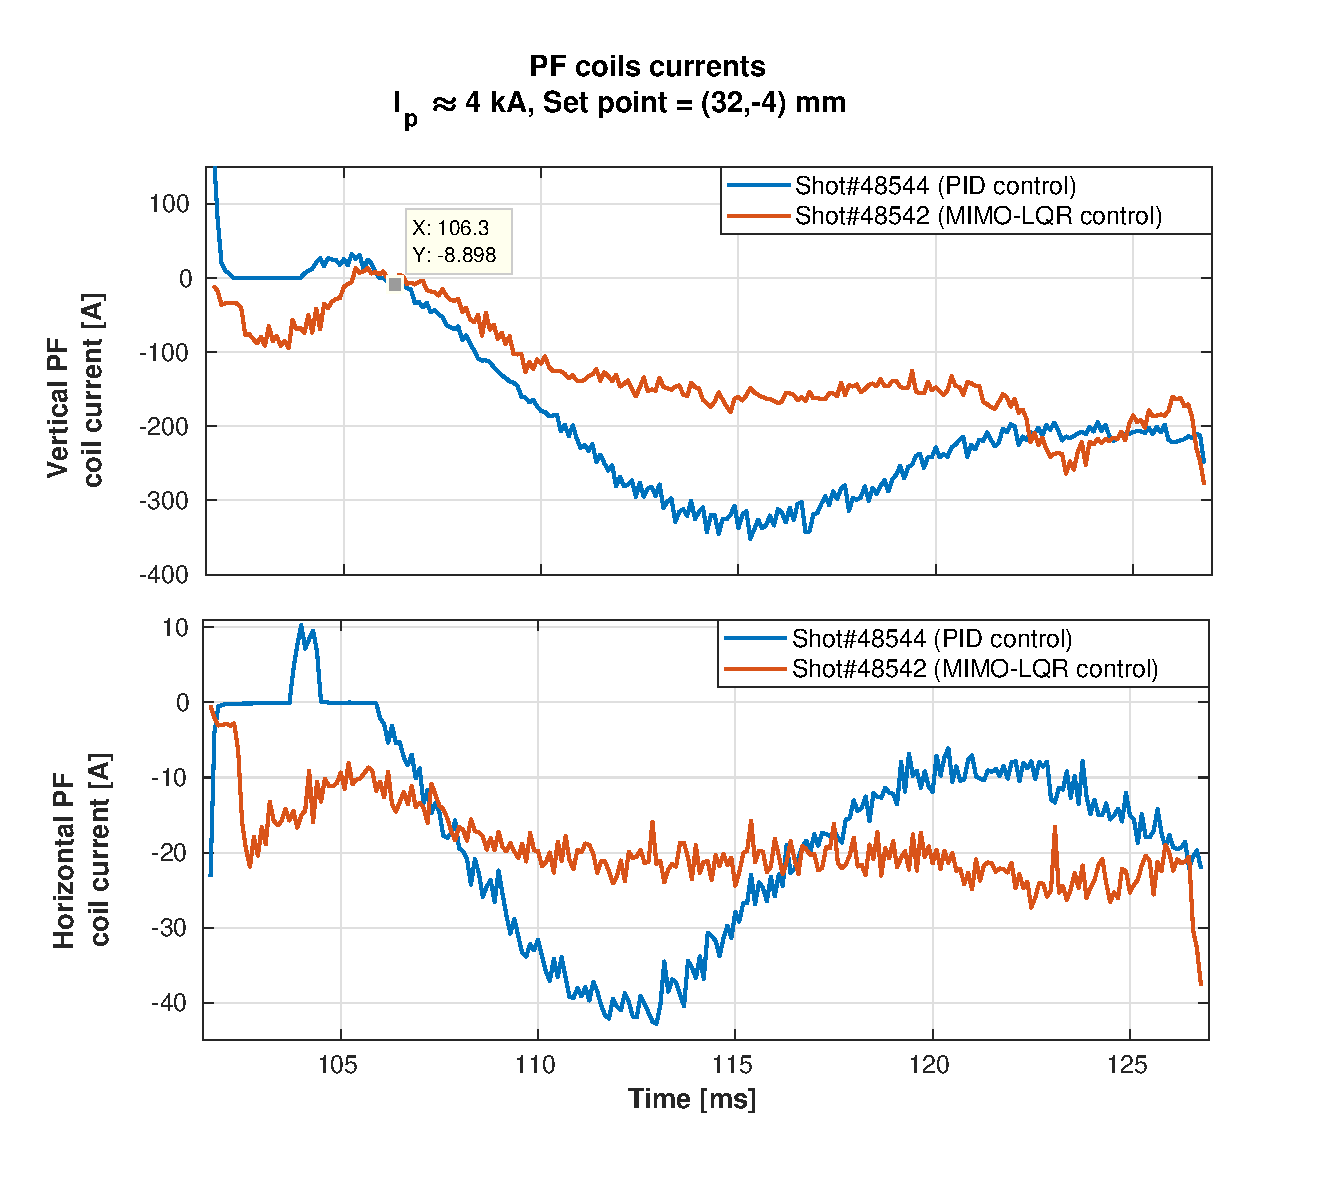
\includegraphics[width=0.7\textwidth]{Chp5/PIDvsMIMO_544_542_curr_2.eps}
	\caption{   Vertical and Horizontal PF coils currents during  $I_p\approx 4kA$  flat-tops. Orange time trace corresponds to a PID feedback control and blue time trace to a LQR MIMO feedback control. Shot $\#$ 48544 and Shot$\#$ 48542.}
\end{figure}

\begin{figure}
	\centering
	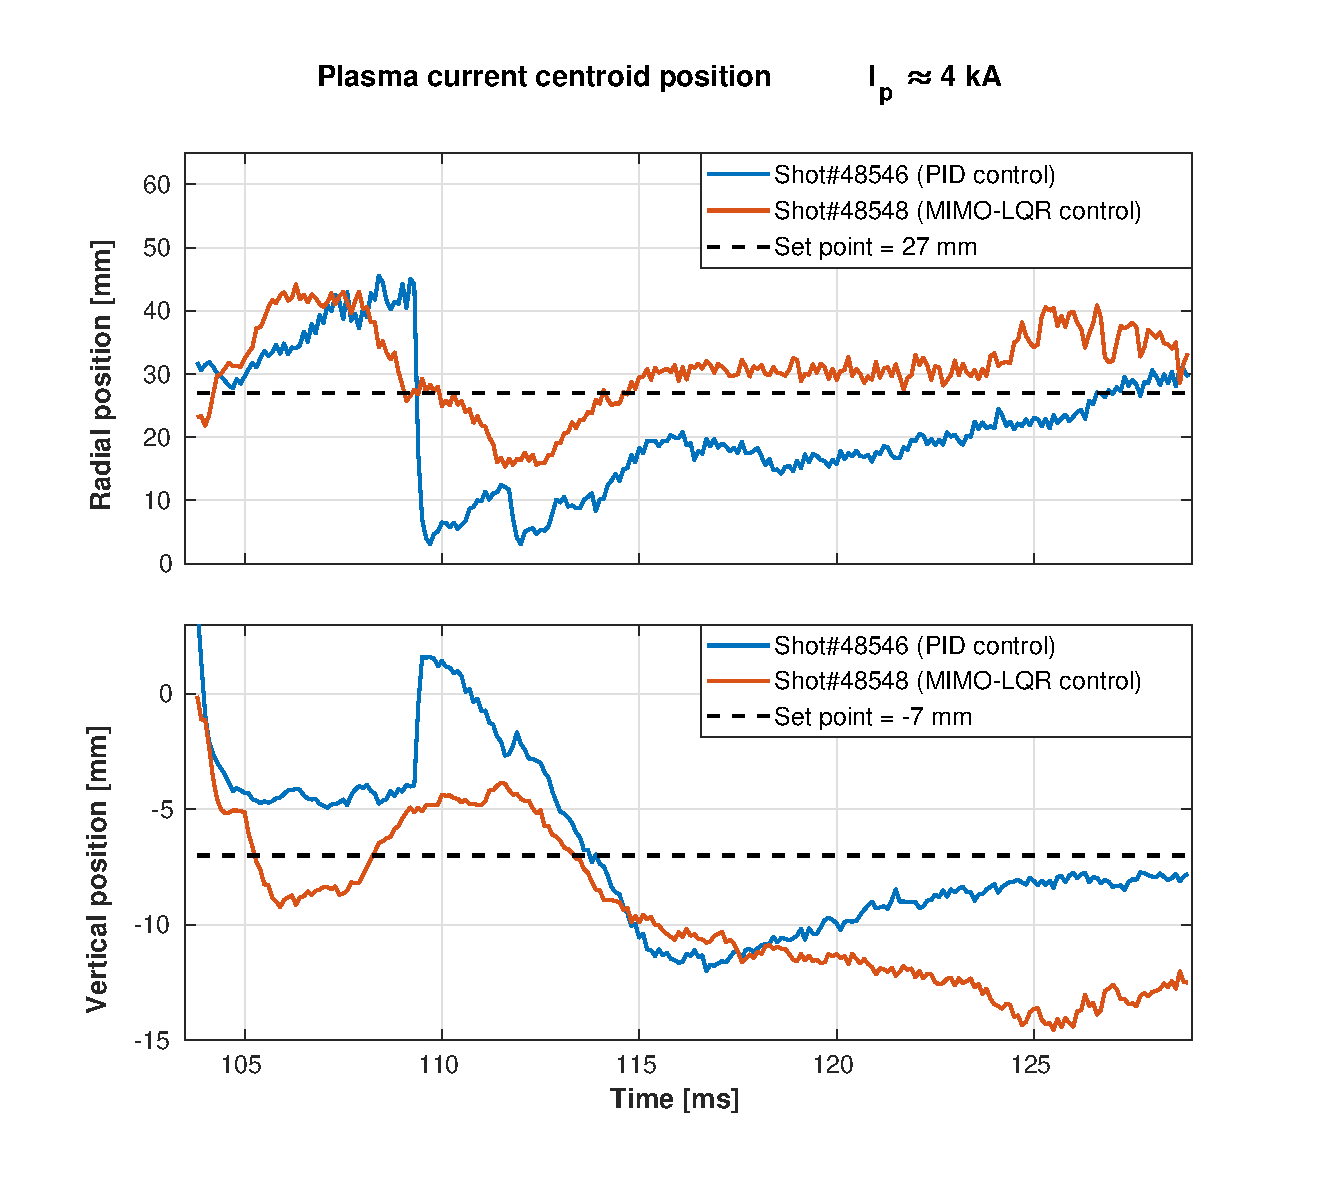
\includegraphics[width=0.7\textwidth]{Chp5/PIDvsMIMO_546_548_2.eps}
	\caption{Horizontal and vertical plasma centroid position during  $I_p\approx 4kA$  flat-tops, orange time trace corresponds to a PID feedback control and blue time trace to a LQR MIMO feedback control, the dashed black line shows the programmed set point.  Shot$ \# $ 48546 and Shot$ \#  $48548.}
\end{figure}

\begin{figure}
	\centering
	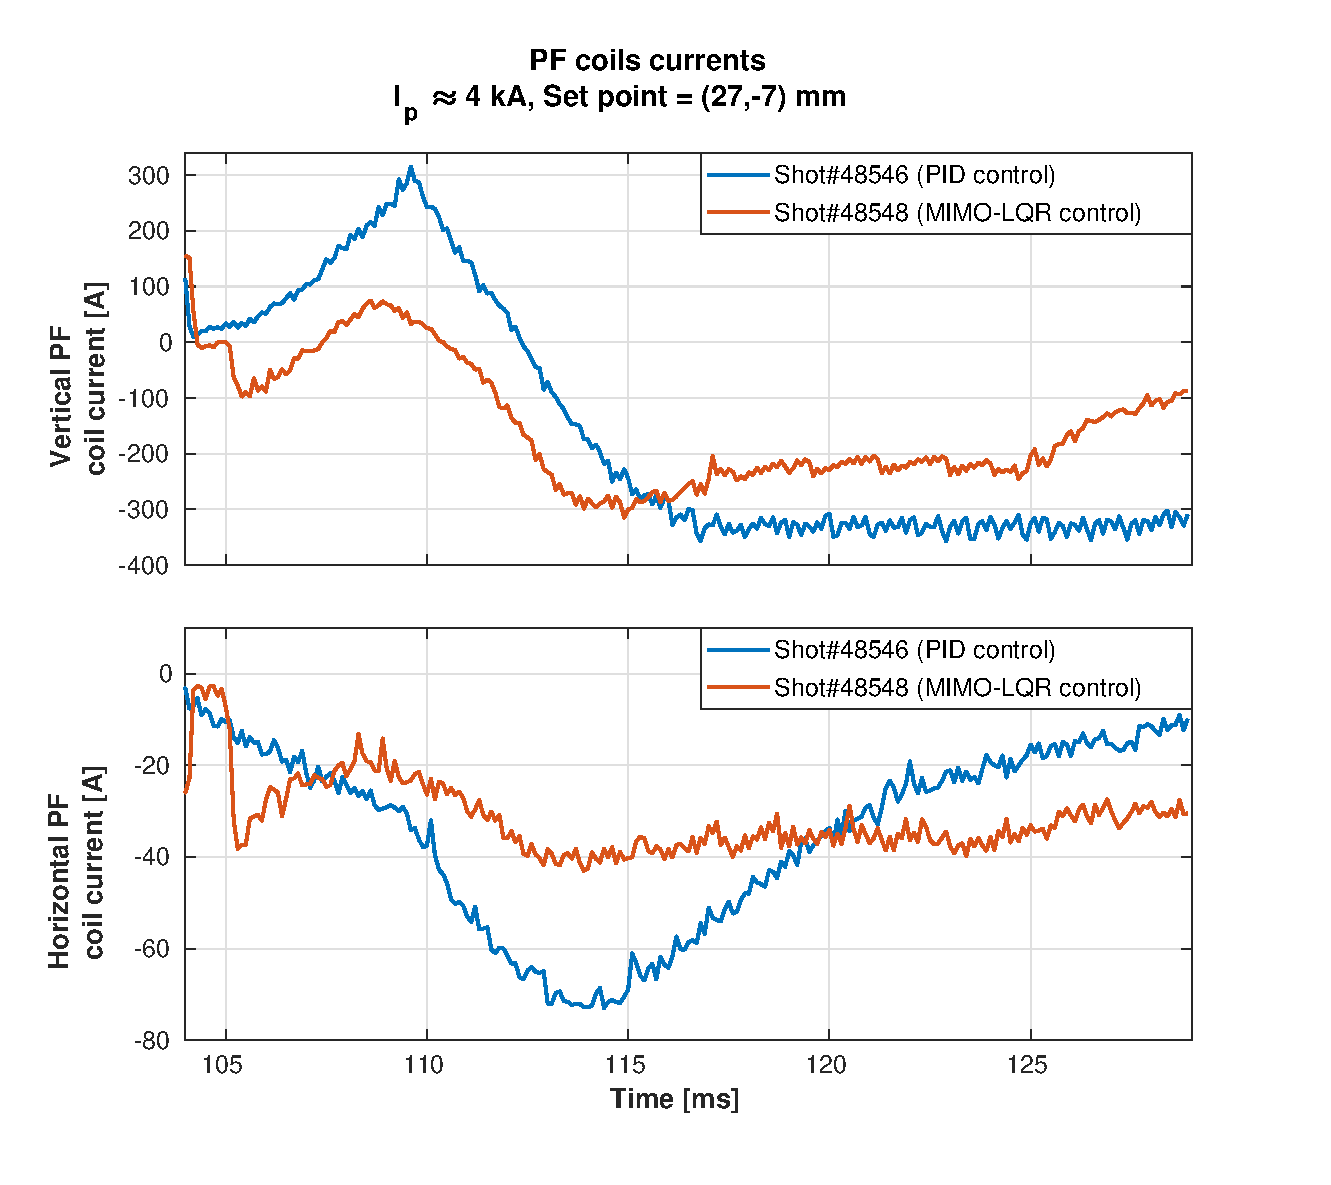
\includegraphics[width=0.7\textwidth]{Chp5/PIDvsMIMO_546_548_curr_2.eps}
	\caption{ Vertical and Horizontal PF coils currents during  $I_p\approx 4kA$  flat-tops. Orange time trace corresponds to a PID feedback control and blue time trace to a LQR MIMO feedback control.  Shot $\#$ 48546 and Shot$\#$ 48548.}
\end{figure}

\begin{figure}
	\centering
	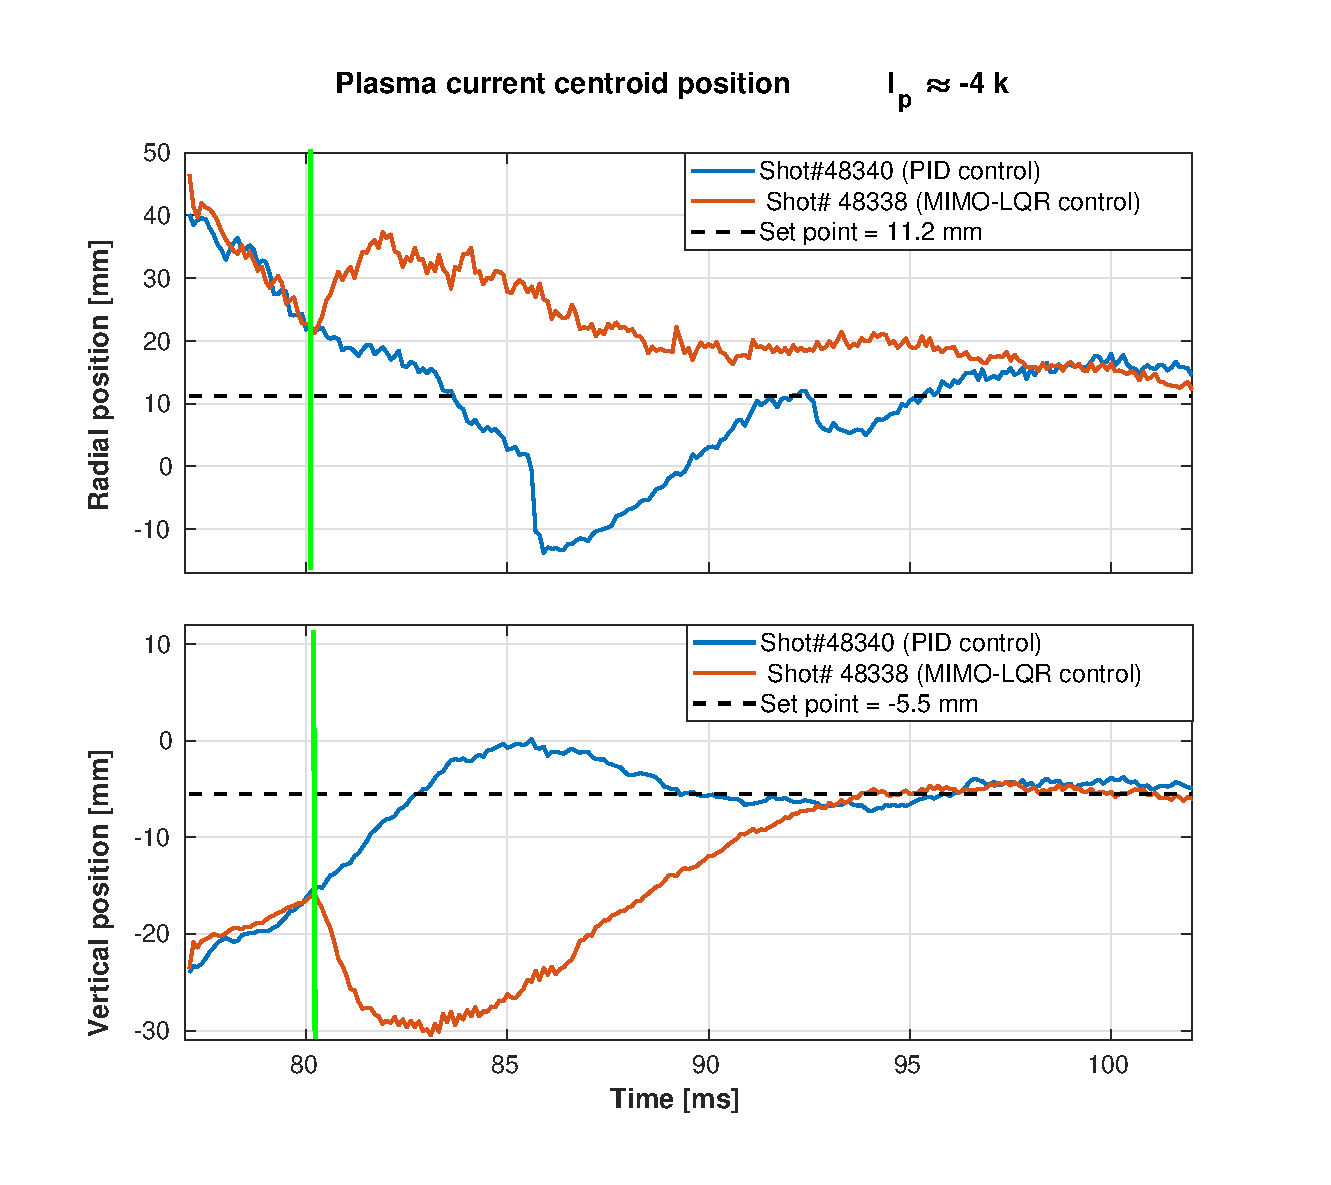
\includegraphics[width=0.67\textwidth]{Chp5/PIDvsMIMO_340_338_2.eps}
	\caption{Horizontal and vertical plasma centroid position during  $I_p\approx 4kA$  flat-tops, orange time trace corresponds to a PID feedback control and blue time trace to a LQR MIMO feedback control, the dashed black line shows the programmed set point. The green vertical line marks the time  when the  discharge Shot$\# ~48338$ switches  from PID to MIMO LQR control.	}
\end{figure}

\begin{figure}
	\centering
	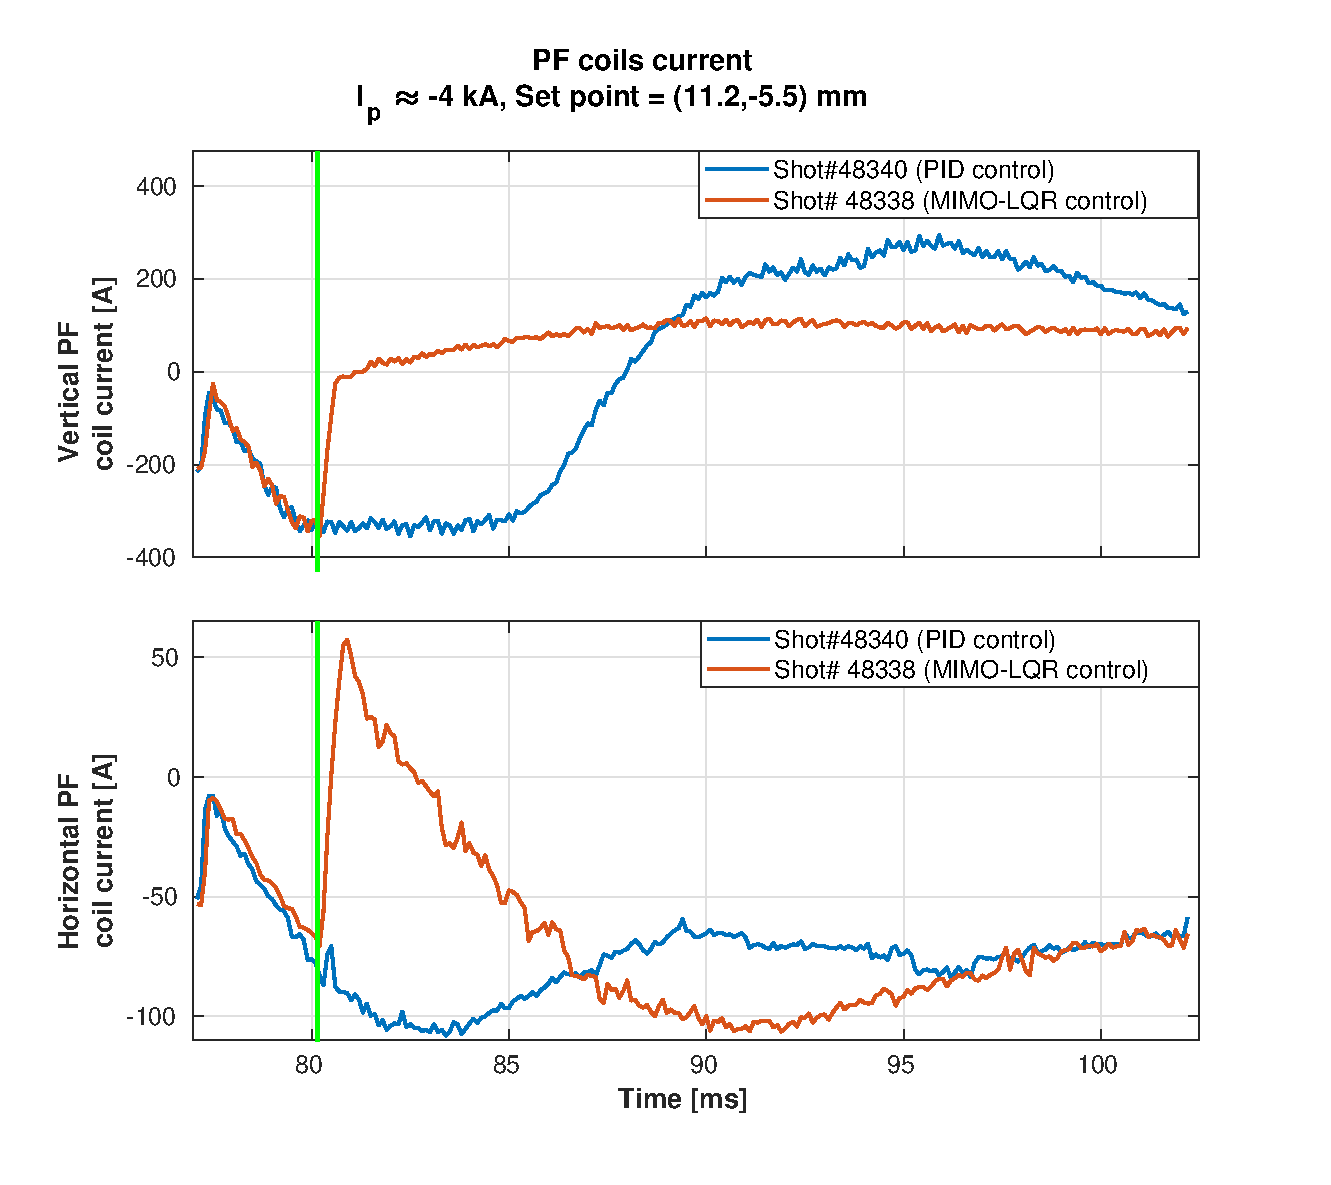
\includegraphics[width=0.67\textwidth]{Chp5/PIDvsMIMO_340_338_curr_2.eps}
	\caption{ Vertical and Horizontal PF coils currents during  $I_p\approx -4kA$  flat-tops. Orange time trace corresponds to a PID feedback control and blue time trace to a LQR MIMO feedback control. The green vertical line marks the time  when the  discharge Shot$\# 48338$ switches the control from PID to MIMO LQR. Shot$\#~$ 48340 and Shot$\#~$ 48338.}
\end{figure}

\begin{figure}
	\centering
	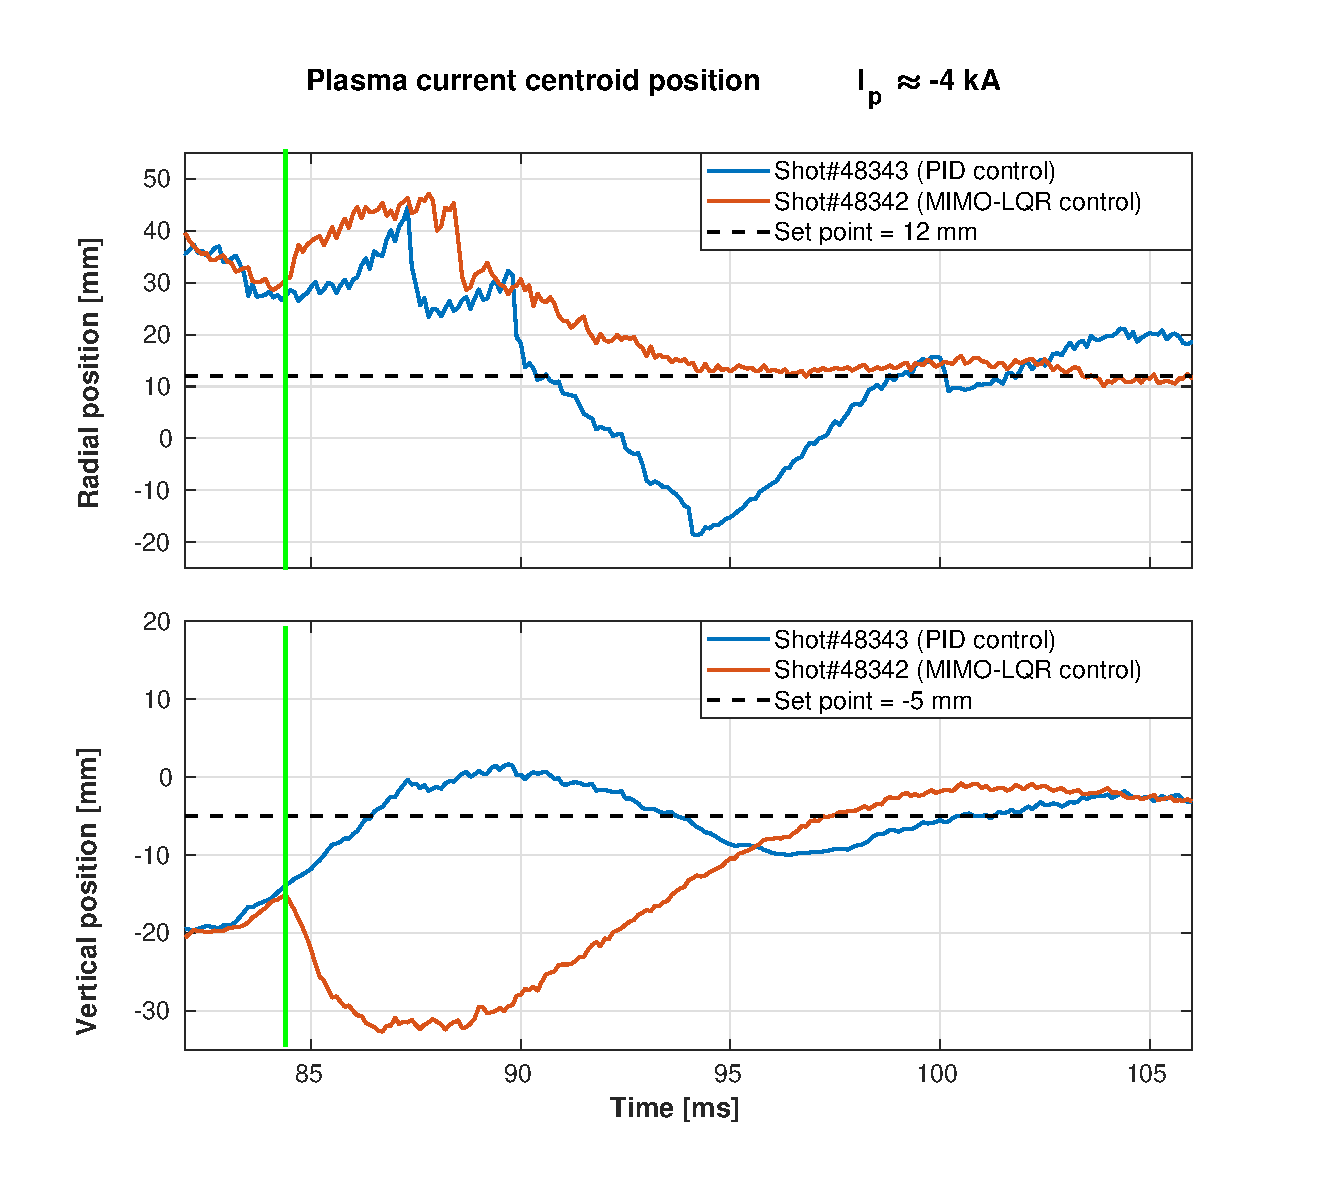
\includegraphics[width=0.67\textwidth]{Chp5/PIDvsMIMO_343_342_2.eps}
	\caption{Horizontal and vertical plasma centroid position during  $I_p\approx 4kA$  flat-tops, orange time trace corresponds to a PID feedback control and blue time trace to a LQR MIMO feedback control, the dashed black line shows the programmed set point. The green vertical line marks the time  when the  discharge Shot$\# ~48342$ switches  from PID to MIMO LQR control.}
\end{figure}

\begin{figure}
	\centering
	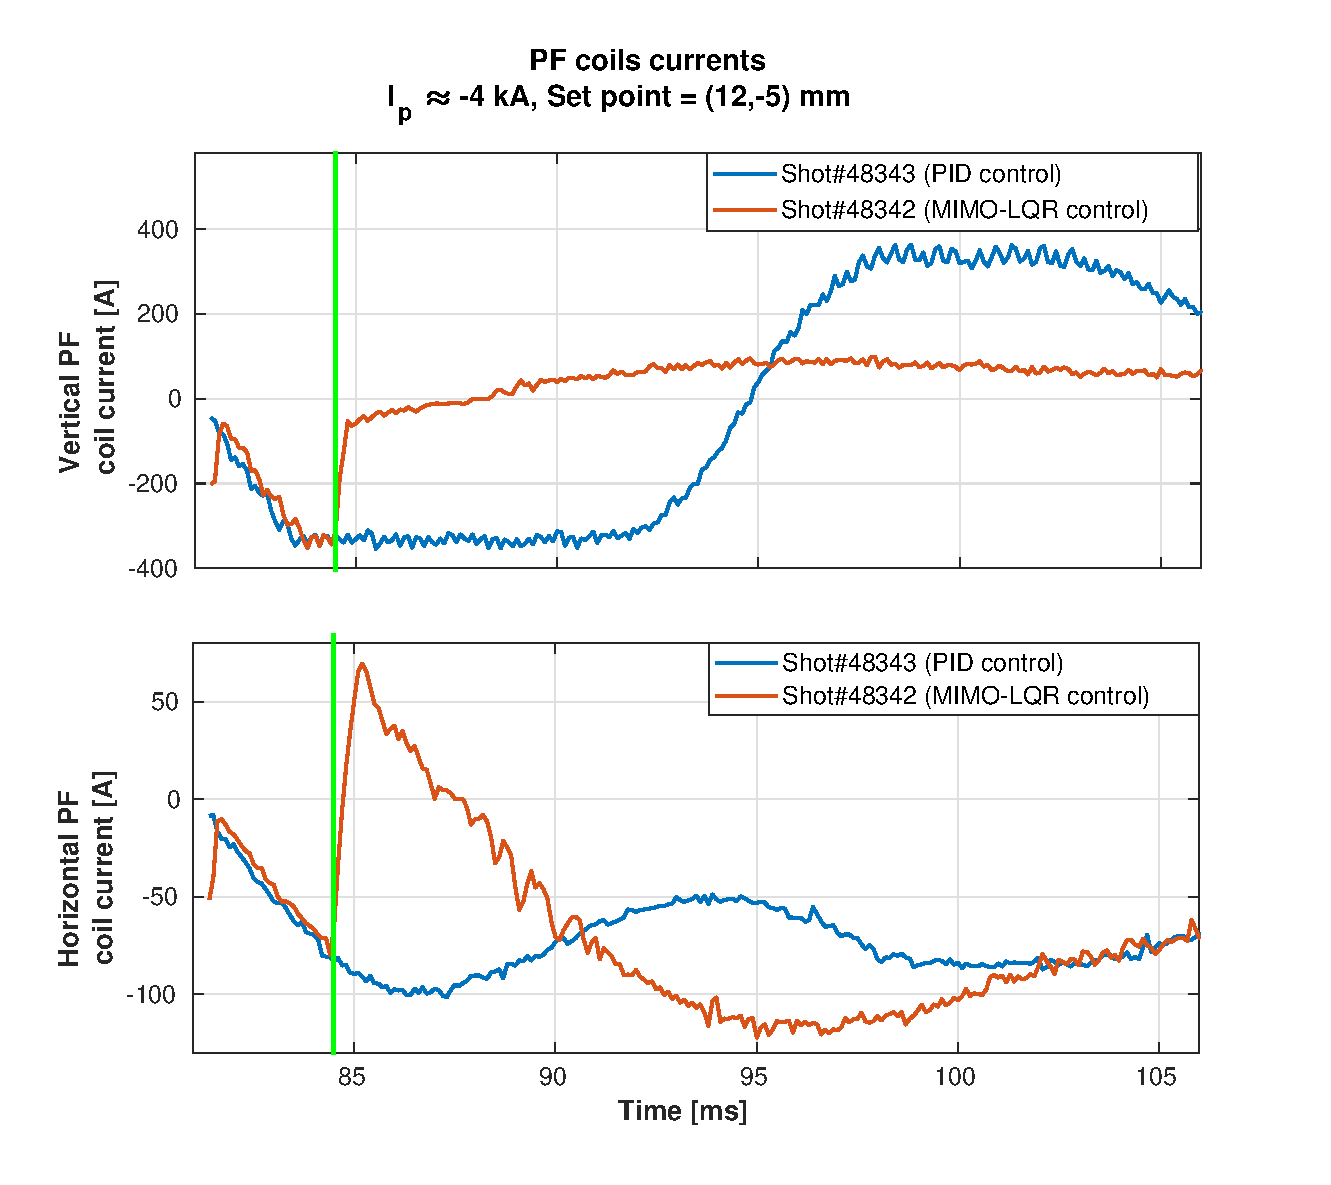
\includegraphics[width=0.67\textwidth]{Chp5/PIDvsMIMO_343_342_curr_2.eps}
	\caption{ Vertical and Horizontal PF coils currents during  $I_p\approx -4kA$  flat-tops. Orange time trace corresponds to a PID feedback control and blue time trace to a LQR MIMO feedback control. The green vertical line marks the time  when the  discharge Shot$\# 48342$ switches the control from PID to MIMO LQR. Shot $\#$ 48343 and Shot$\#$ 48342.}
\end{figure}

\begin{figure}
	\centering
	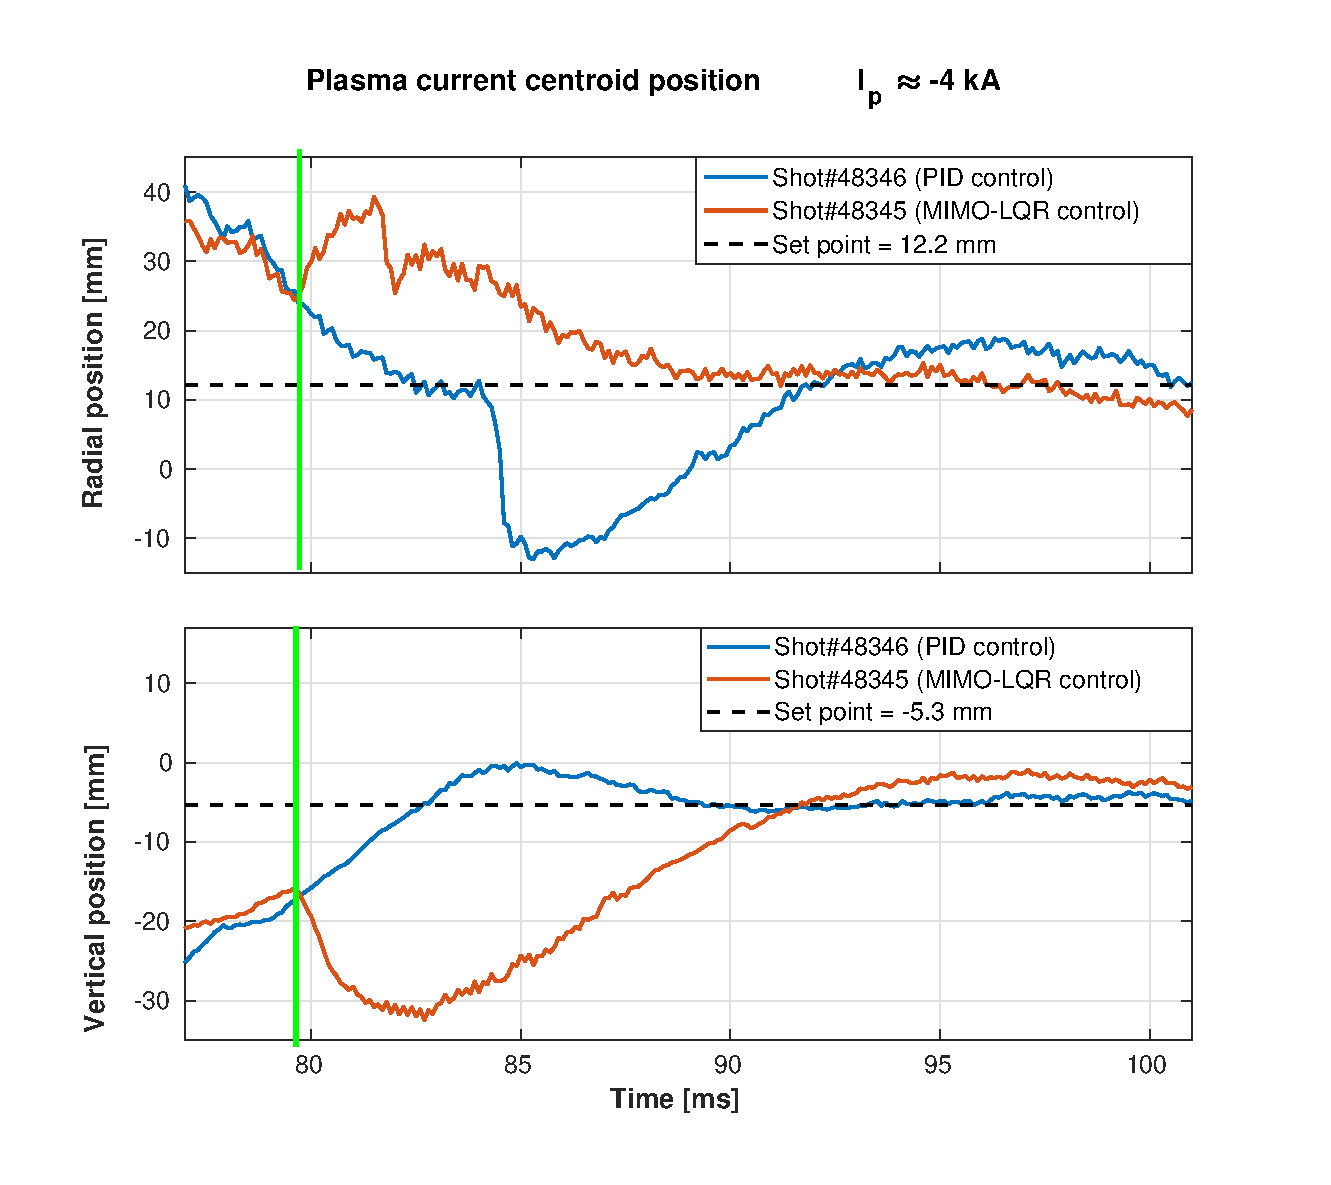
\includegraphics[width=0.67\textwidth]{Chp5/PIDvsMIMO_346_345_2.eps}
	\caption{Horizontal and vertical plasma centroid position during  $I_p\approx 4kA$  flat-tops, orange time trace corresponds to a PID feedback control and blue time trace to a LQR MIMO feedback control, the dashed black line shows the programmed set point. The green vertical line marks the time  when the  discharge Shot$\# ~48345$ switches  from PID to MIMO LQR control.}
\end{figure}

\begin{figure}
	\centering
	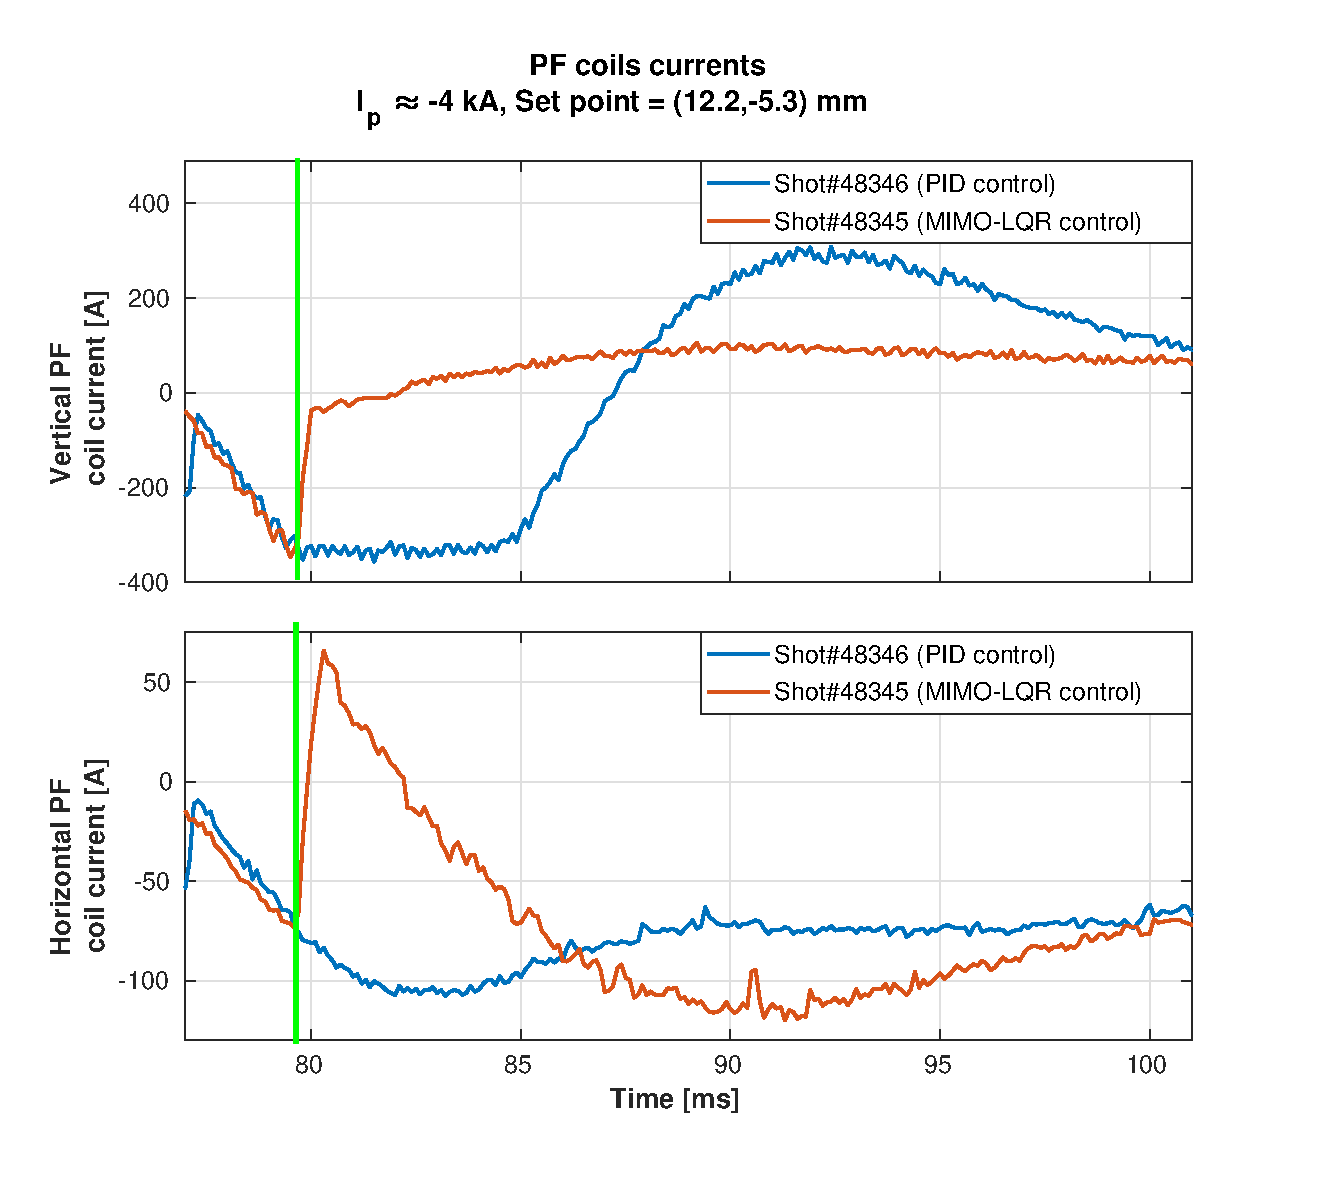
\includegraphics[width=0.67\textwidth]{Chp5/PIDvsMIMO_346_345_curr_2.eps}
	\caption{Vertical and Horizontal PF coils currents during  $I_p\approx -4kA$  flat-tops. Orange time trace corresponds to a PID feedback control and blue time trace to a LQR MIMO feedback control. The green vertical line marks the time  when the  discharge Shot$\# 48345$ switches the control from PID to MIMO LQR.  Shot$\#$  48346 and  Shot$\#$ 48345.}
\end{figure}

\begin{figure}
	\centering
	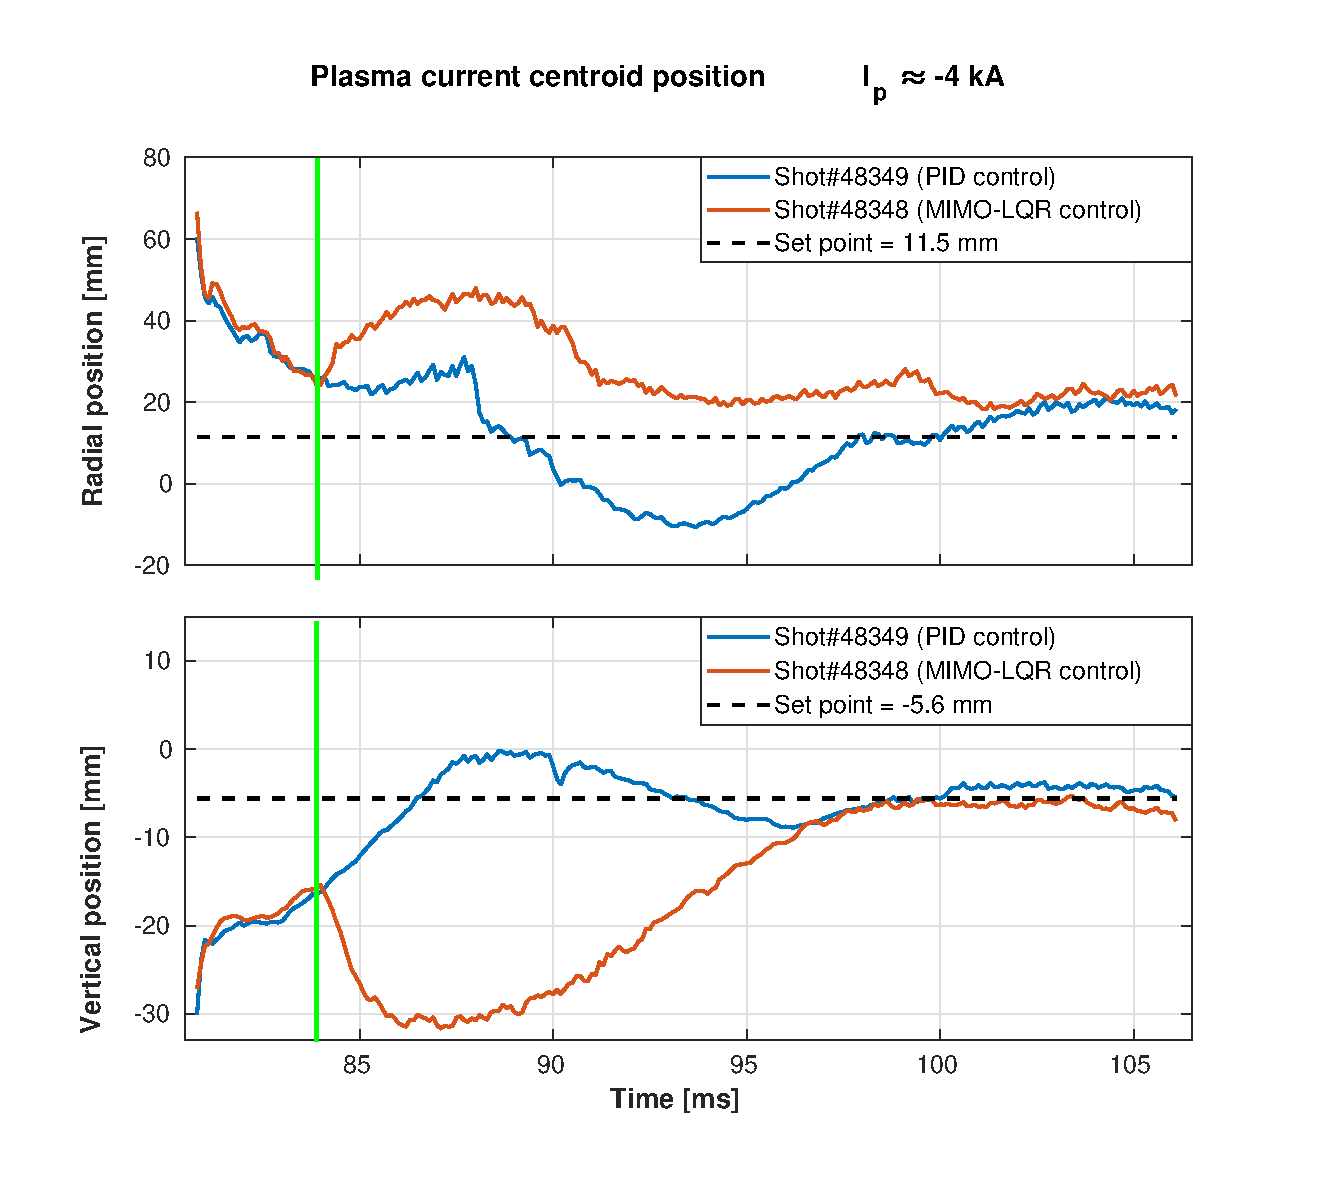
\includegraphics[width=0.67\textwidth]{Chp5/PIDvsMIMO_349_348_2.eps}
	\caption{Horizontal and vertical plasma centroid position during  $I_p\approx 4kA$  flat-tops, orange time trace corresponds to a PID feedback control and blue time trace to a LQR MIMO feedback control, the dashed black line shows the programmed set point. The green vertical line marks the time  when the  discharge Shot$\# ~48348$ switches  from PID to MIMO LQR control.}
\end{figure}

\begin{figure}
	\centering
	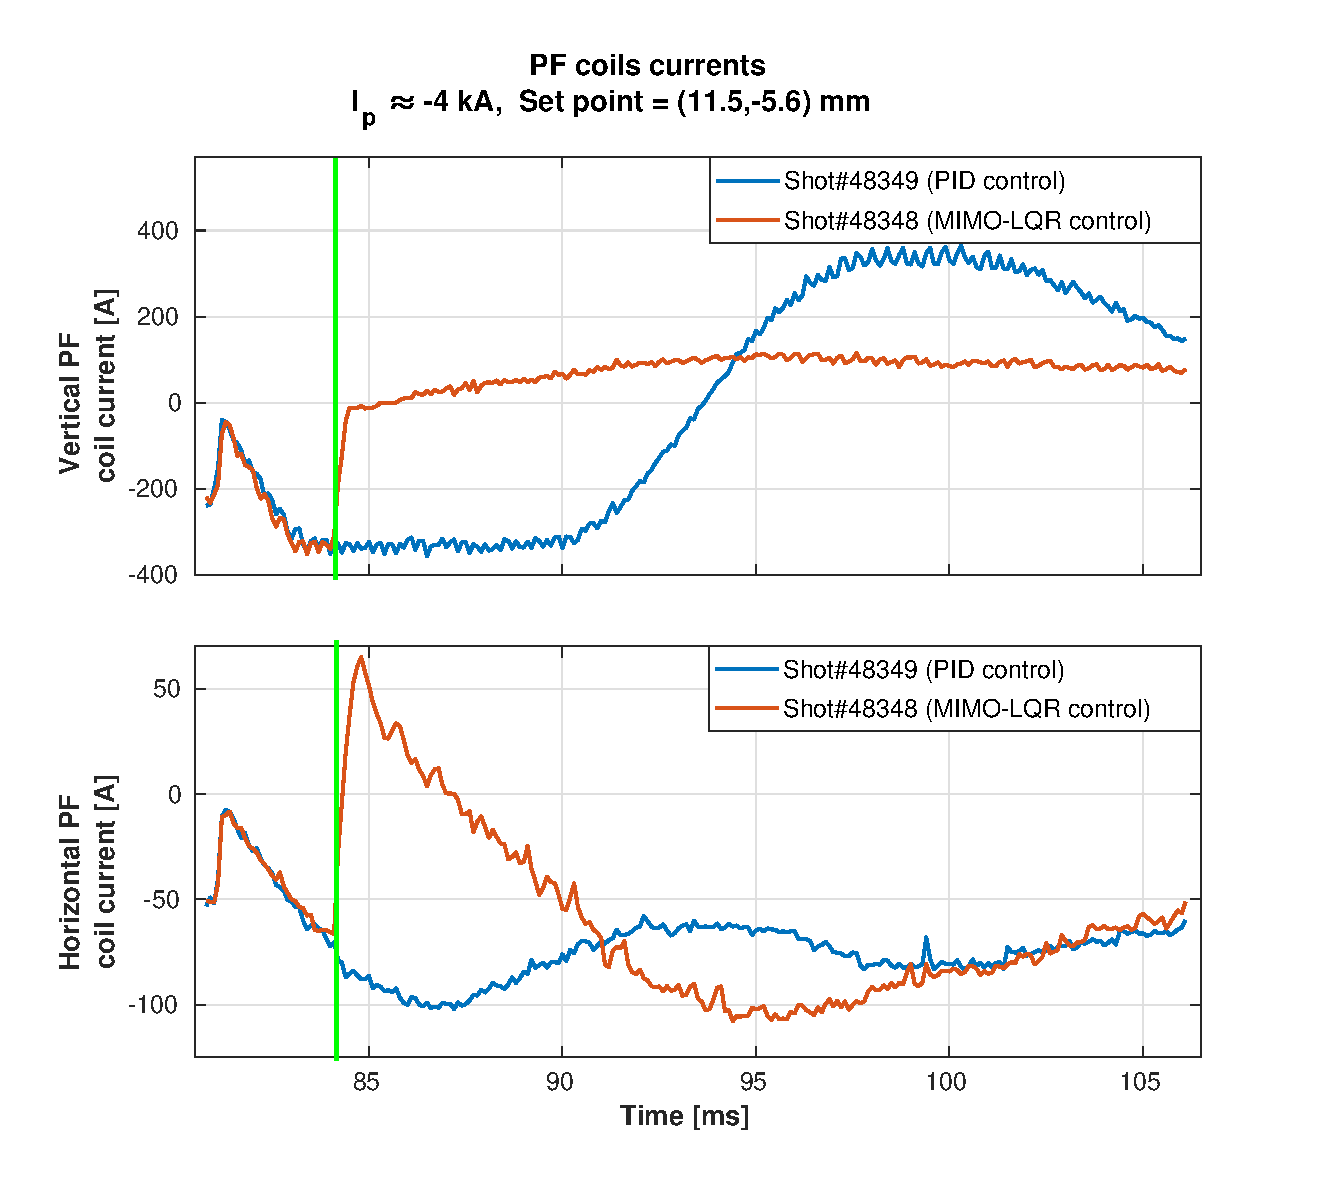
\includegraphics[width=0.67\textwidth]{Chp5/PIDvsMIMO_349_348_curr_2.eps}
	\caption{ Vertical and Horizontal PF coils currents during  $I_p\approx -4kA$  flat-tops. Orange time trace corresponds to a PID feedback control and blue time trace to a LQR MIMO feedback control. The green vertical line marks the time  when the  discharge Shot$\# 48348$ switches the control from PID to MIMO LQR. Shot$\#$ 48349 and Shot$\#$ 48348}
\end{figure}


\begin{figure}
	\centering
	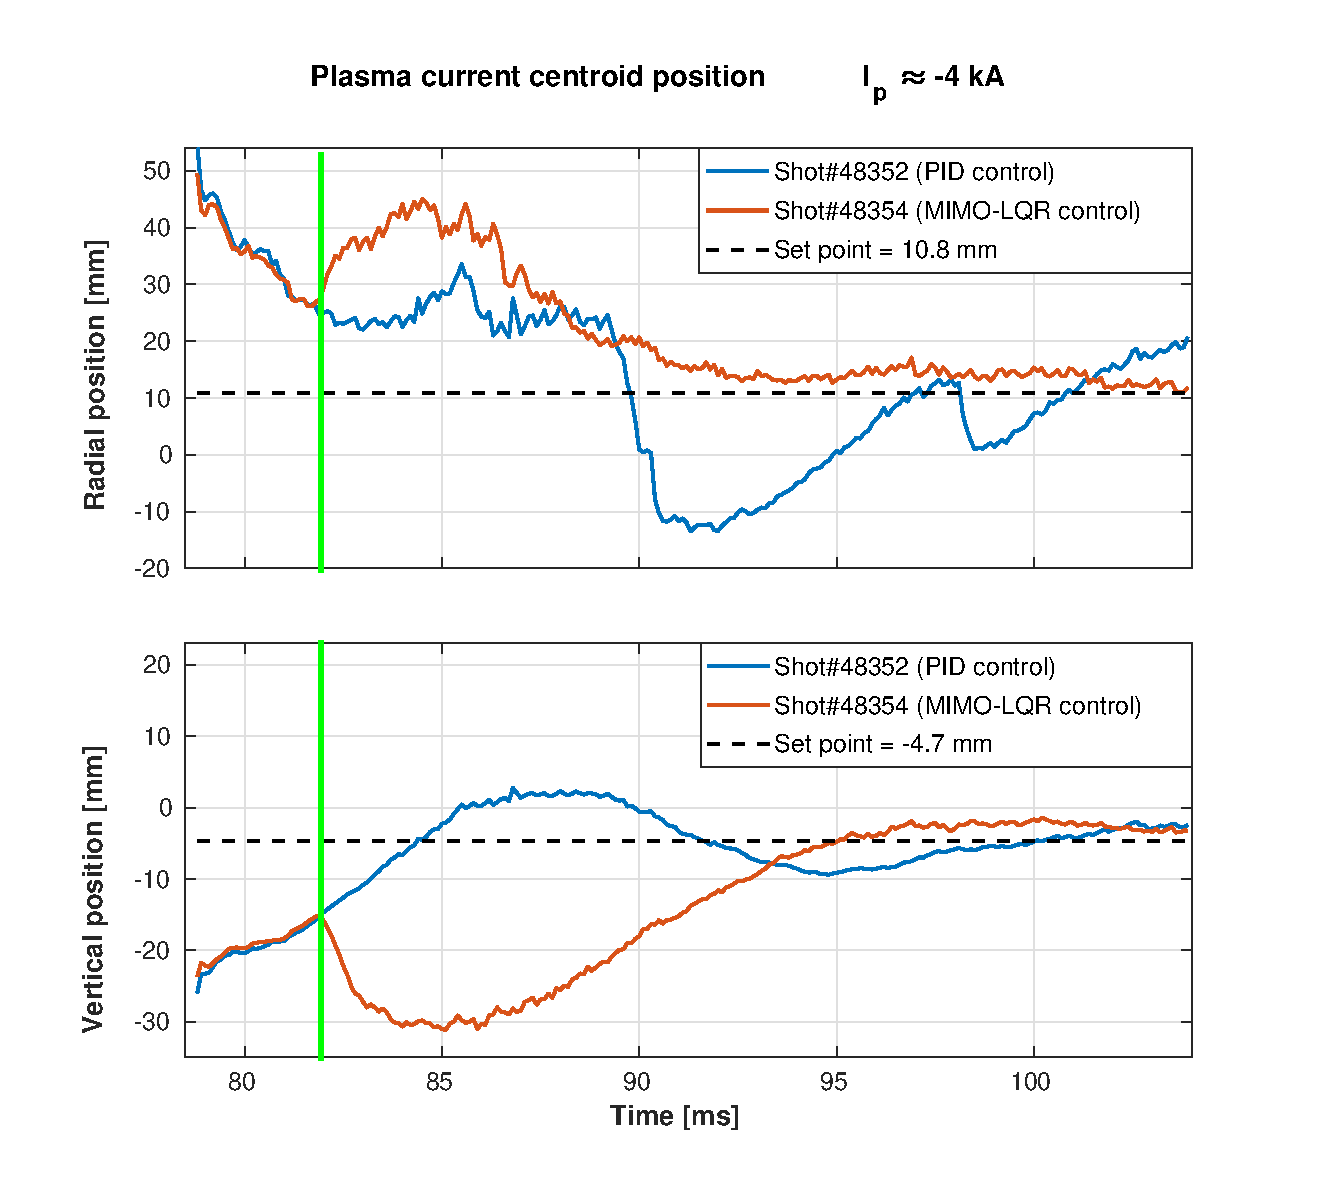
\includegraphics[width=0.67\textwidth]{Chp5/PIDvsMIMO_352_354_2.eps}
	\caption{Horizontal and vertical plasma centroid position during  $I_p\approx 4kA$  flat-tops, orange time trace corresponds to a PID feedback control and blue time trace to a LQR MIMO feedback control, the dashed black line shows the programmed set point. The green vertical line marks the time  when the  discharge Shot$\# ~48354$ switches  from PID to MIMO LQR control.}
\end{figure}

\begin{figure}
	\centering
	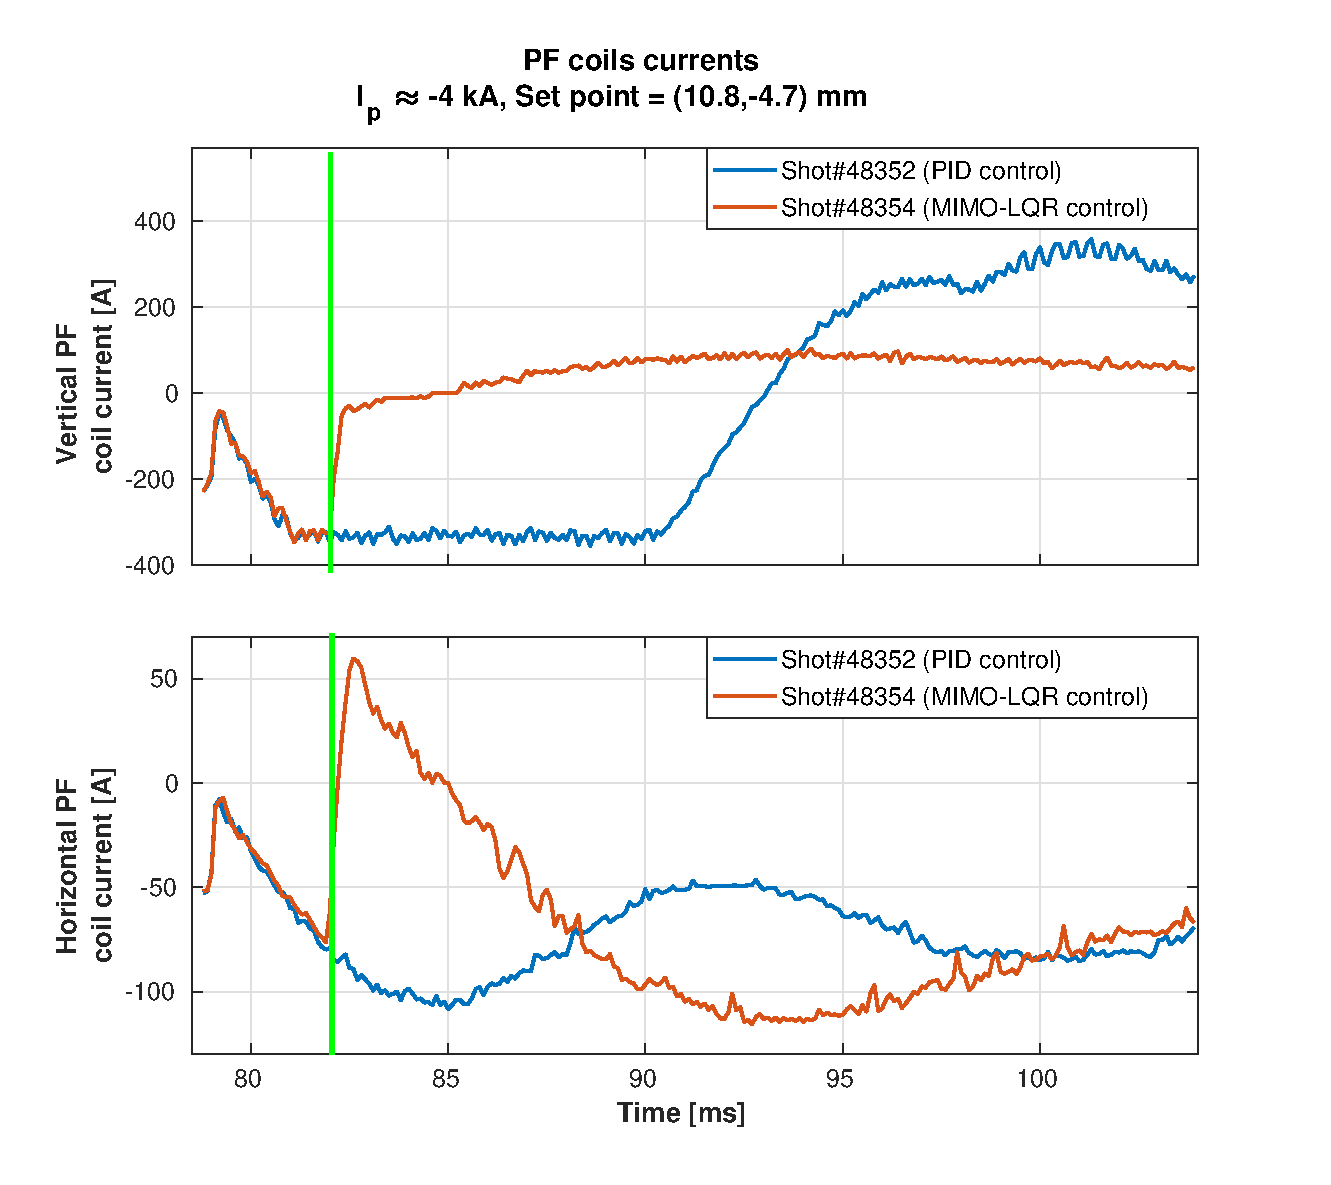
\includegraphics[width=0.67\textwidth]{Chp5/PIDvsMIMO_352_354_curr_2.eps}
	\caption{ Vertical and Horizontal PF coils currents during  $I_p\approx -4kA$  flat-tops. Orange time trace corresponds to a PID feedback control and blue time trace to a LQR MIMO feedback control. The green vertical line marks the time  when the  discharge Shot$\# 48354$ switches the control from PID to MIMO LQR. Shot$\#$ 48352 and Shot$\#$ 48354.}
\end{figure}


\begin{figure}
	\centering
	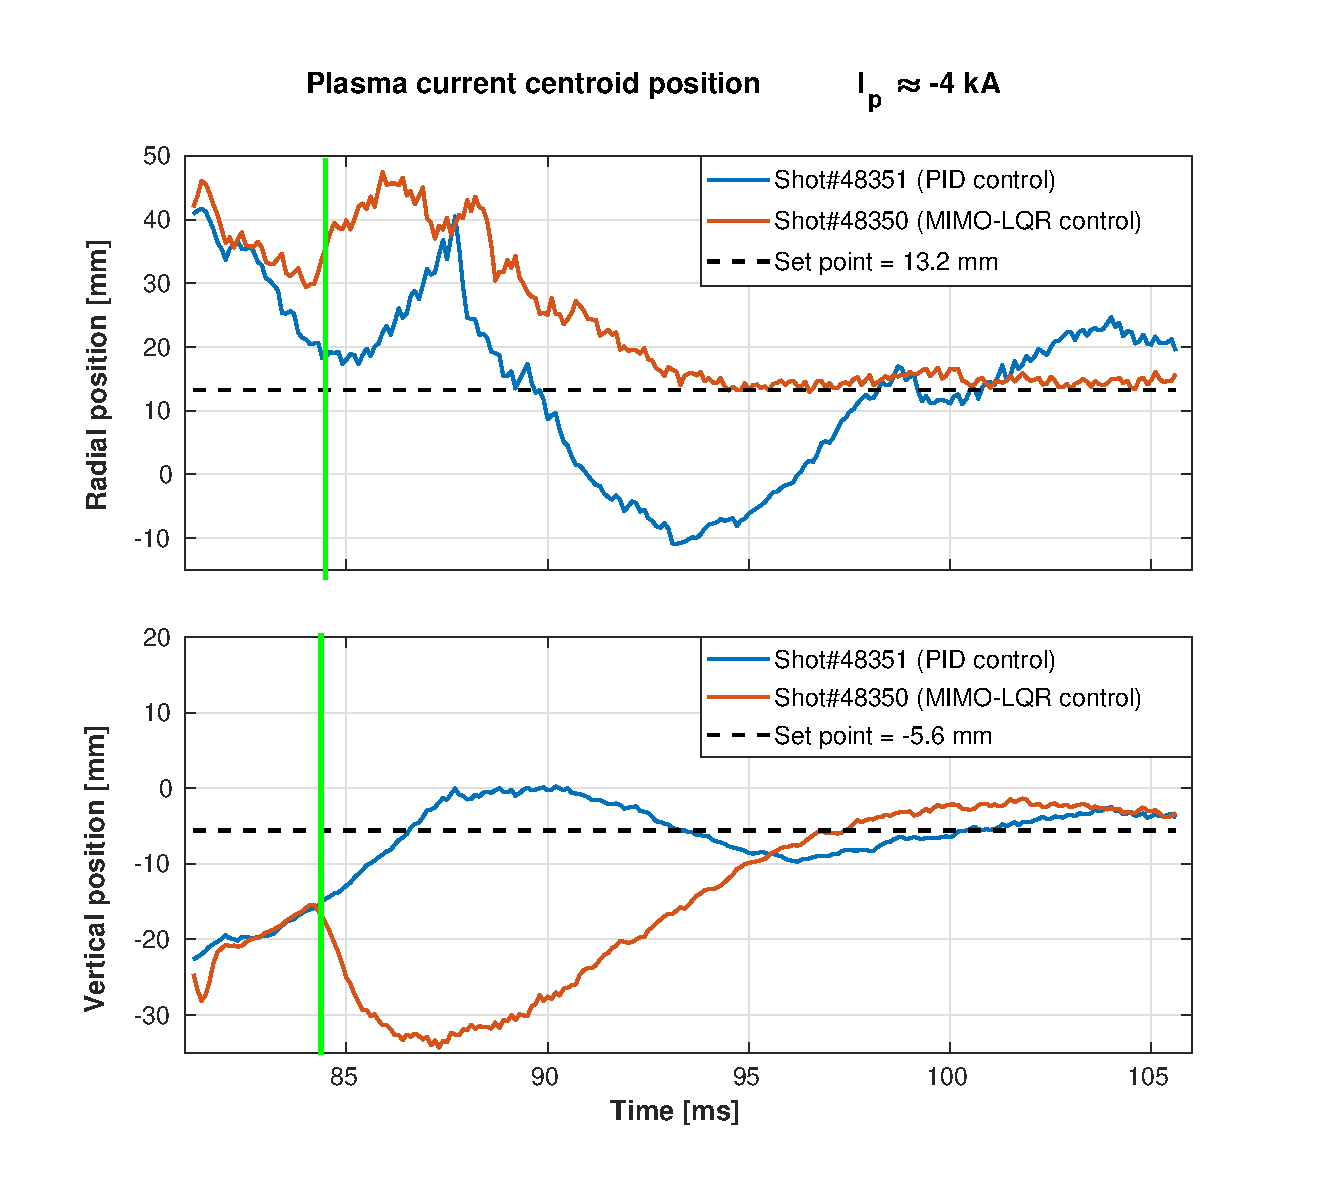
\includegraphics[width=0.67\textwidth]{Chp5/PIDvsMIMO_351_350_2.eps}
	\caption{Horizontal and vertical plasma centroid position during  $I_p\approx 4kA$  flat-tops, orange time trace corresponds to a PID feedback control and blue time trace to a LQR MIMO feedback control, the dashed black line shows the programmed set point. The green vertical line marks the time  when the  discharge Shot$\# ~48350$ switches  from PID to MIMO LQR control.}
\end{figure}

\begin{figure}
	\centering
	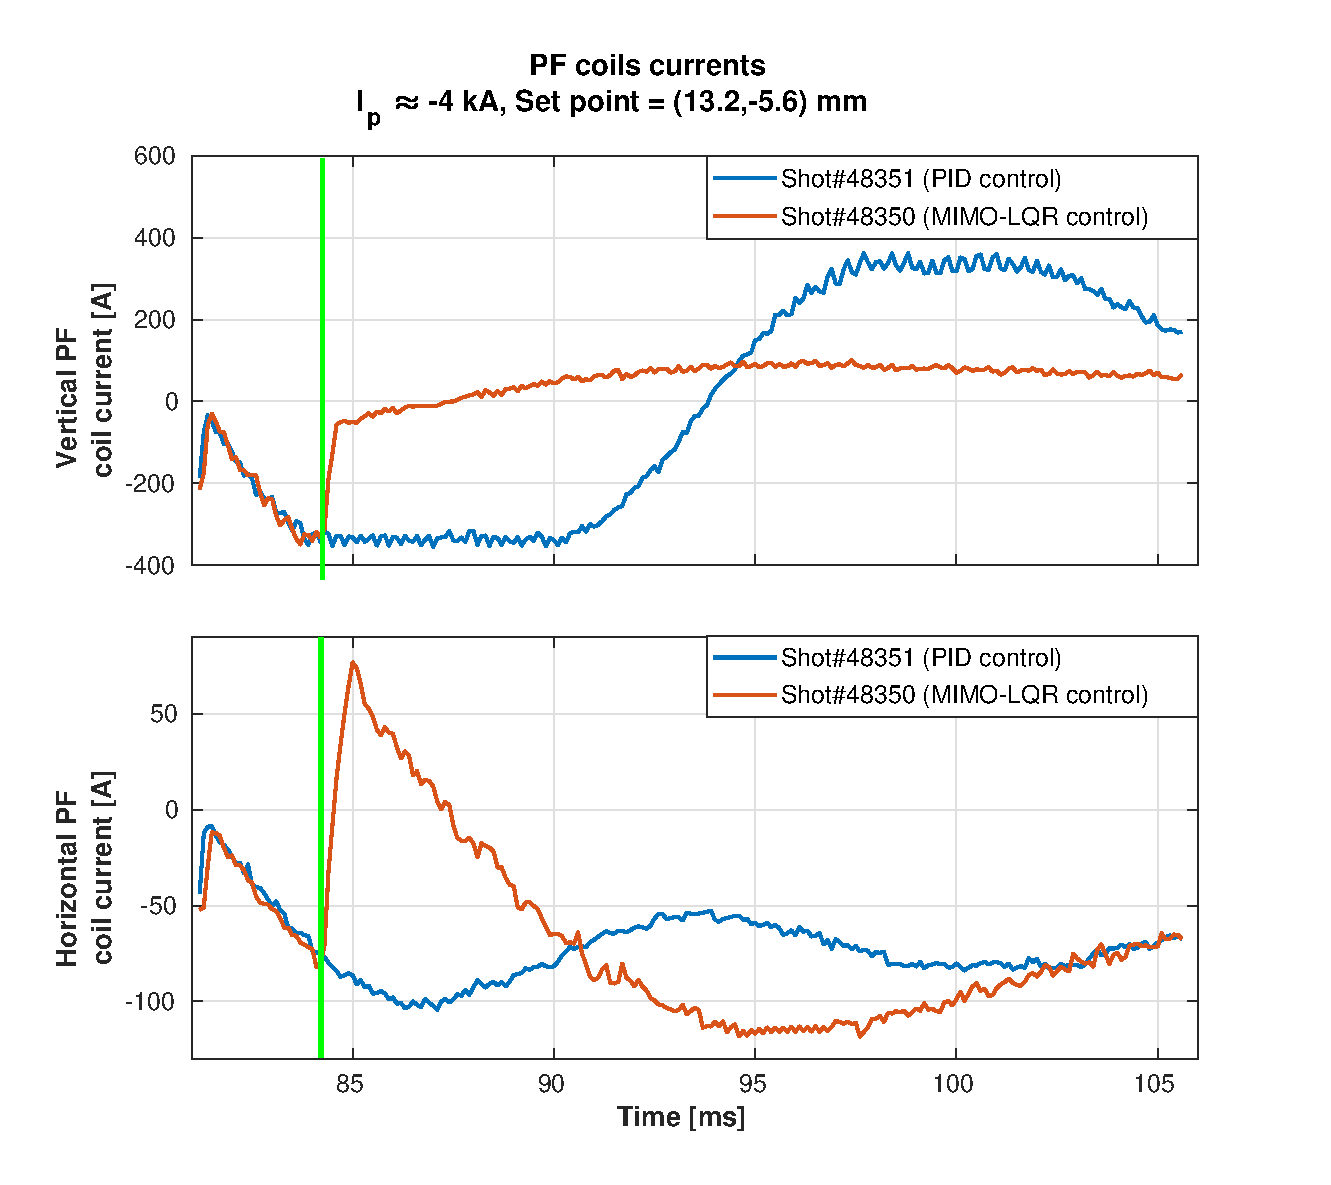
\includegraphics[width=0.67\textwidth]{Chp5/PIDvsMIMO_351_350_curr_2.eps}
	\caption{Vertical and Horizontal PF coils currents during  $I_p\approx -4kA$  flat-tops. Orange time trace corresponds to a PID feedback control and blue time trace to a LQR MIMO feedback control. The green vertical line marks the time  when the  discharge Shot$\# 48350$ switches the control from PID to MIMO LQR.  Shot$\#$ 48351 and Shot$\#$ 48350.}
\end{figure}